\documentclass{article}

\usepackage{ctex}
\usepackage{fancyhdr}
\usepackage{extramarks}
\usepackage{amsmath}
\usepackage{amsthm}
\usepackage{amssymb} 
\usepackage{amsfonts}
\usepackage{tikz}
\usepackage{url}
\usepackage{float}


%\usetikzlibrary{automata,positioning}

%
% Basic Document Settings
%

\topmargin=-0.45in
\evensidemargin=0in
\oddsidemargin=0in
\textwidth=6.5in
\textheight=9.0in
\headsep=0.25in


\pagestyle{fancy}
\lhead{\hmwkAuthorName}
\chead{\hmwkClass\ (\hmwkClassInstructor): \hmwkTitle}
\rhead{\schoolID}
\lfoot{}
\cfoot{\thepage}

\renewcommand\headrulewidth{0.4pt}
\renewcommand\footrulewidth{0.4pt}

\setlength\parindent{0pt}

%
% Create Problem Sections
%

\newcommand{\enterProblemHeader}[1]{
    \nobreak\extramarks{}{Problem \arabic{#1} continued on next page\ldots}\nobreak{}
    \nobreak\extramarks{Problem \arabic{#1} (continued)}{Problem \arabic{#1} continued on next page\ldots}\nobreak{}
}

\newcommand{\exitProblemHeader}[1]{
    \nobreak\extramarks{Problem \arabic{#1} (continued)}{Problem \arabic{#1} continued on next page\ldots}\nobreak{}
    \stepcounter{#1}
    \nobreak\extramarks{Problem \arabic{#1}}{}\nobreak{}
}

\setcounter{secnumdepth}{0}
\newcounter{partCounter}
\newcounter{homeworkProblemCounter}
\setcounter{homeworkProblemCounter}{1}
\nobreak\extramarks{Problem \arabic{homeworkProblemCounter}}{}\nobreak{}

%
% Homework Problem Environment
%
% This environment takes an optional argument. When given, it will adjust the
% problem counter. This is useful for when the problems given for your
% assignment aren't sequential. See the last 3 problems of this template for an
% example.
%
\newenvironment{homeworkProblem}[1][-1]{
    \ifnum#1>0
        \setcounter{homeworkProblemCounter}{#1}
    \fi
    \section{Problem \arabic{homeworkProblemCounter}}
    \setcounter{partCounter}{1}
    \enterProblemHeader{homeworkProblemCounter}
}{
    \exitProblemHeader{homeworkProblemCounter}
}

%
% Homework Details
%   - Title
%   - Due date
%   - Class
%   - Section/Time
%   - Instructor
%   - Author
%

\newcommand{\hmwkTitle}{Homework\ \#6}
\newcommand{\hmwkClass}{Pattern Recognition}
\newcommand{\hmwkClassInstructor}{Professor Wang Guijin}
\newcommand{\hmwkAuthorName}{{Qingyun~Fang} }
\newcommand{\schoolID}{{2017311003}}

\newcommand{\hs}{\hspace{2em}}
\newcommand{\vs}{\vspace{2ex}}
%
% Title Page
%

\title{
    \vspace{2in}
    \textmd{\textbf{\hmwkClass:\ \hmwkTitle}}\\
    %\normalsize\vspace{0.1in}\small{Due\ on\ \hmwkDueDate\ at 3:10pm}\\
    \vspace{0.5cm}\LARGE{\textit{\hmwkClassInstructor}}
    \vspace{4in}
}

\author{\hmwkAuthorName\\
{\schoolID}\\
Use \LaTeX ~in 5.2~2018} 


\date{}

\renewcommand{\part}[1]{\textbf{ Part \Alph{partCounter}}\stepcounter{partCounter}}

%
% Various Helper Commands
%


% Alias for the Solution section header
\newcommand{\solution}{\textbf{\Large Solution}}

% Probability commands: Expectation, Variance, Covariance, Bias
\newcommand{\E}{\mathrm{E}}
\newcommand{\Var}{\mathrm{Var}}
\newcommand{\Cov}{\mathrm{Cov}}
\newcommand{\Bias}{\mathrm{Bias}}

\linespread{1.5}

\begin{document}

\maketitle
\setcounter{page}{0}
\thispagestyle{empty}
\pagebreak

\section{Problem One}
{\kaishu{\large KNN算法}}

\hs 问题背景:有两组二维数据,在空间中的样本分布如 图1所示。对一个新的样本点,请尝试用KNN算法判断 它的所属组别。

\begin{figure}[htbp]
	\centering
	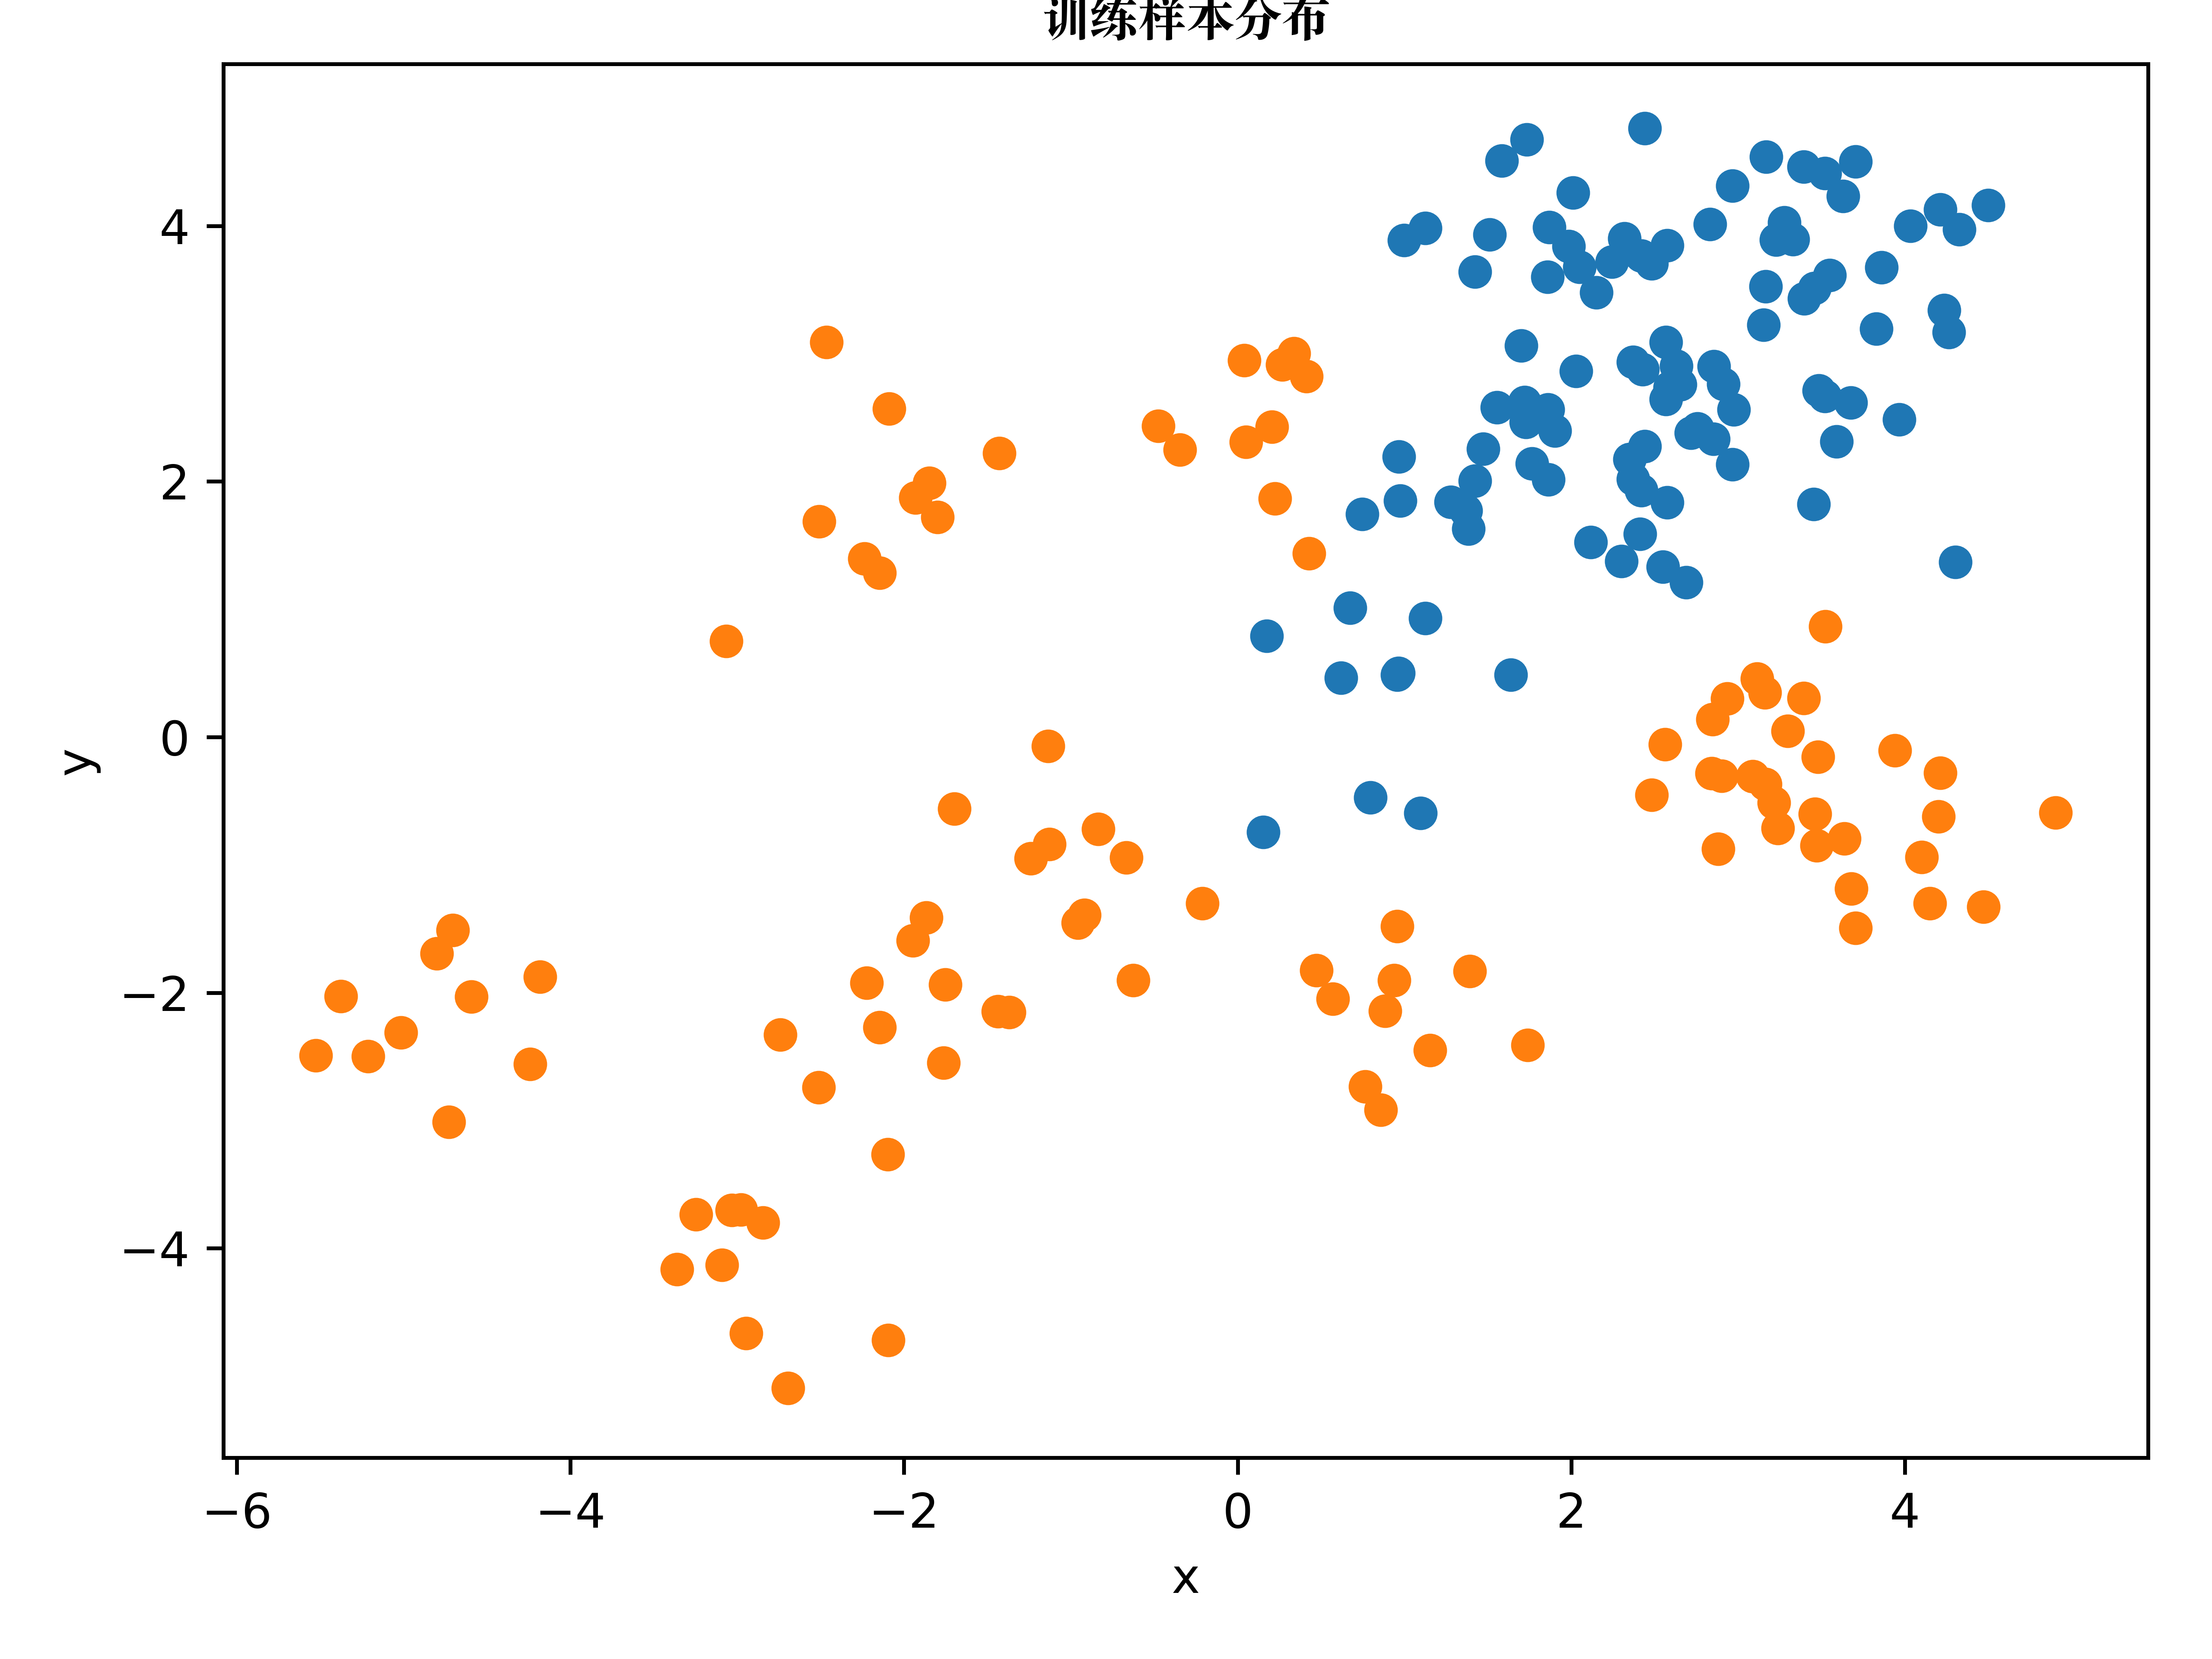
\includegraphics[width=0.6\linewidth]{img//fig1.png}
	\caption{训练样本}
\end{figure}

{\kaishu{\large 算法理解}}

\hs 在很多情况下,使用最近邻(即把决策建立在最近的样本上)的方法具有一定的风险,特别是当样本分布复杂或者是数据噪声较大的时候。K-近邻算法就是在最近邻的基础上引入了投票机制,选择离样本最近的$k$个已知的样本,用他们的类别进行投票来决定新样本的类别。值得注意的是,对于两类问题,如果在这些$k$个样本的权重是一样的话,那么$k$必然需要选择一个奇数,从而避免对两类投票出现票数相同的情况。

\hs K-近邻法可以表示为:设有N个已知的样本分属于c个类($\omega_i,i=1,2,...,c$),考察新样本$ x$在这些样本中的前$k$个近邻,设其中有$k_i$个属于$\omega_i$类,则$\omega_i$类的判别函数为:

\begin{equation*}
g_i(x)=k_i, ~~i=1,\dots,c
\end{equation*}

\hs 决策的规则如下:
\begin{equation*}
\text{若}g_k(x)=\max_{i=1,\dots,c}g_i(x),~~\text{则}x\in \omega_k
\end{equation*}\\


\subsection{KNN算法实验结果分析}
{\kaishu{\large precision、recall分析}}

\hs 为了验证KNN算法的有效性,这里我对训练样本集进行了拆分,随机选取训练样本“trainData.txt”中的80\%作为样本训练,其余的20\%为测试集。

\hs 设定KNN的参数如下:$k=5$, weights=uniform(即这$k$个近邻的权重都一致,在做预测时一视同仁),选取5次随机拆分测试集,分别用KNN得到其precision、recall和f1-score后,再取平均,最终的结果如下表1:


\begin{table}[htbp]
	\caption{precision、recall和f1-score统计表}
	\centering
\begin{tabular}{c|cccc}	
	& precision&recall&f1-score & support \\
	\hline
	1    &   1.00  &    0.95  &    0.98  &      22\\
	2    &   0.95    &  1.00   &   0.97    &    18 \\
	avg / total    &   0.98  &    0.97  &    0.98 &       40
\end{tabular}	
\end{table}

\hs 从上表中可以看出,KNN算法无论是精确度还是召回率上来讲都是很高的,在80\%的训练样本下,在测试集中精度可以达到98\%,召回率可以达到97\%,这两个结果都十分优秀,这也说明了KNN算法是一种对于分类问题十分有效的算法。

\hs 其训练分类的结果以及分类的边界如下:

\begin{figure}[htbp]
	\centering
	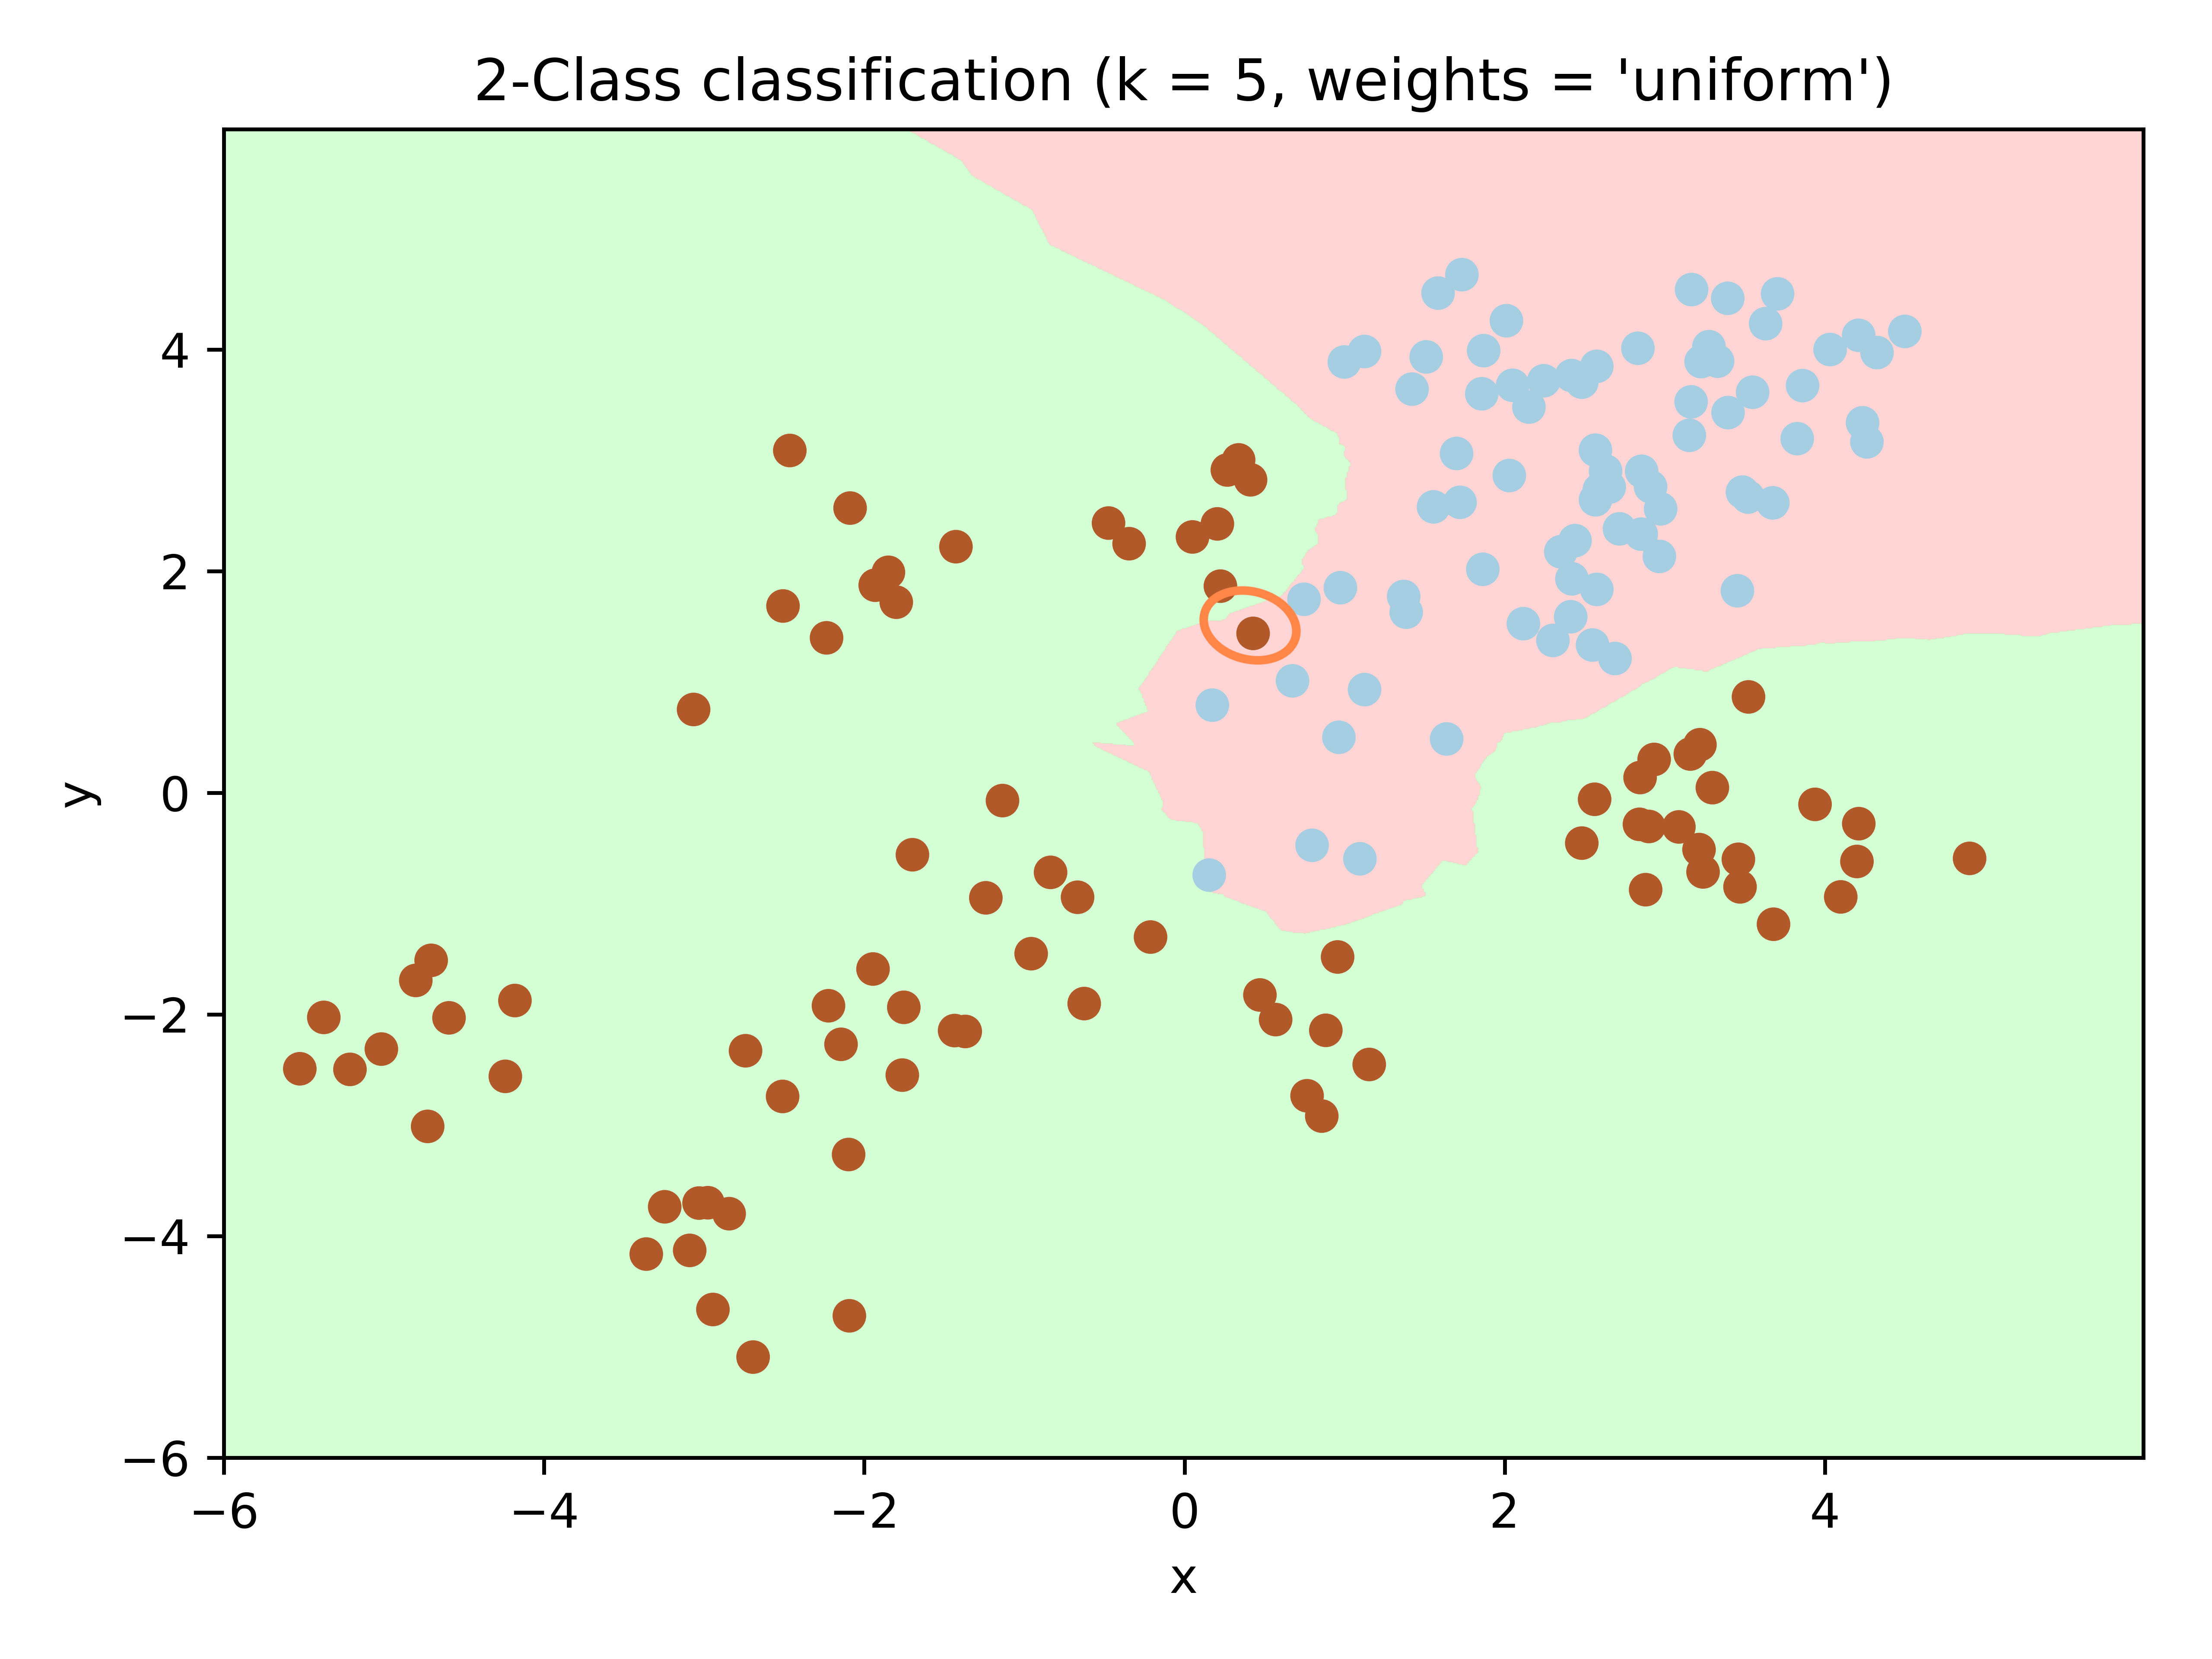
\includegraphics[width=0.6\linewidth]{img//fig6.png}
	\caption{KNN训练分类结果}
\end{figure}

\hs 在上图用橘色框中标记出了一个比较特殊的点,属于“2”类(颜色为棕色),但是却在“1”类(颜色为灰色)的红色区域内,我们可以认为这是一个噪点,并且假设这个点是测试集中的点,那么很显然这个点会被判别到“1”类,这一点我们也可以看其周围的点的分布看出。

\hs 其所有数据的分类结果(浅色为测试集,深色为训练集):

\begin{figure}[htbp]
	\centering
	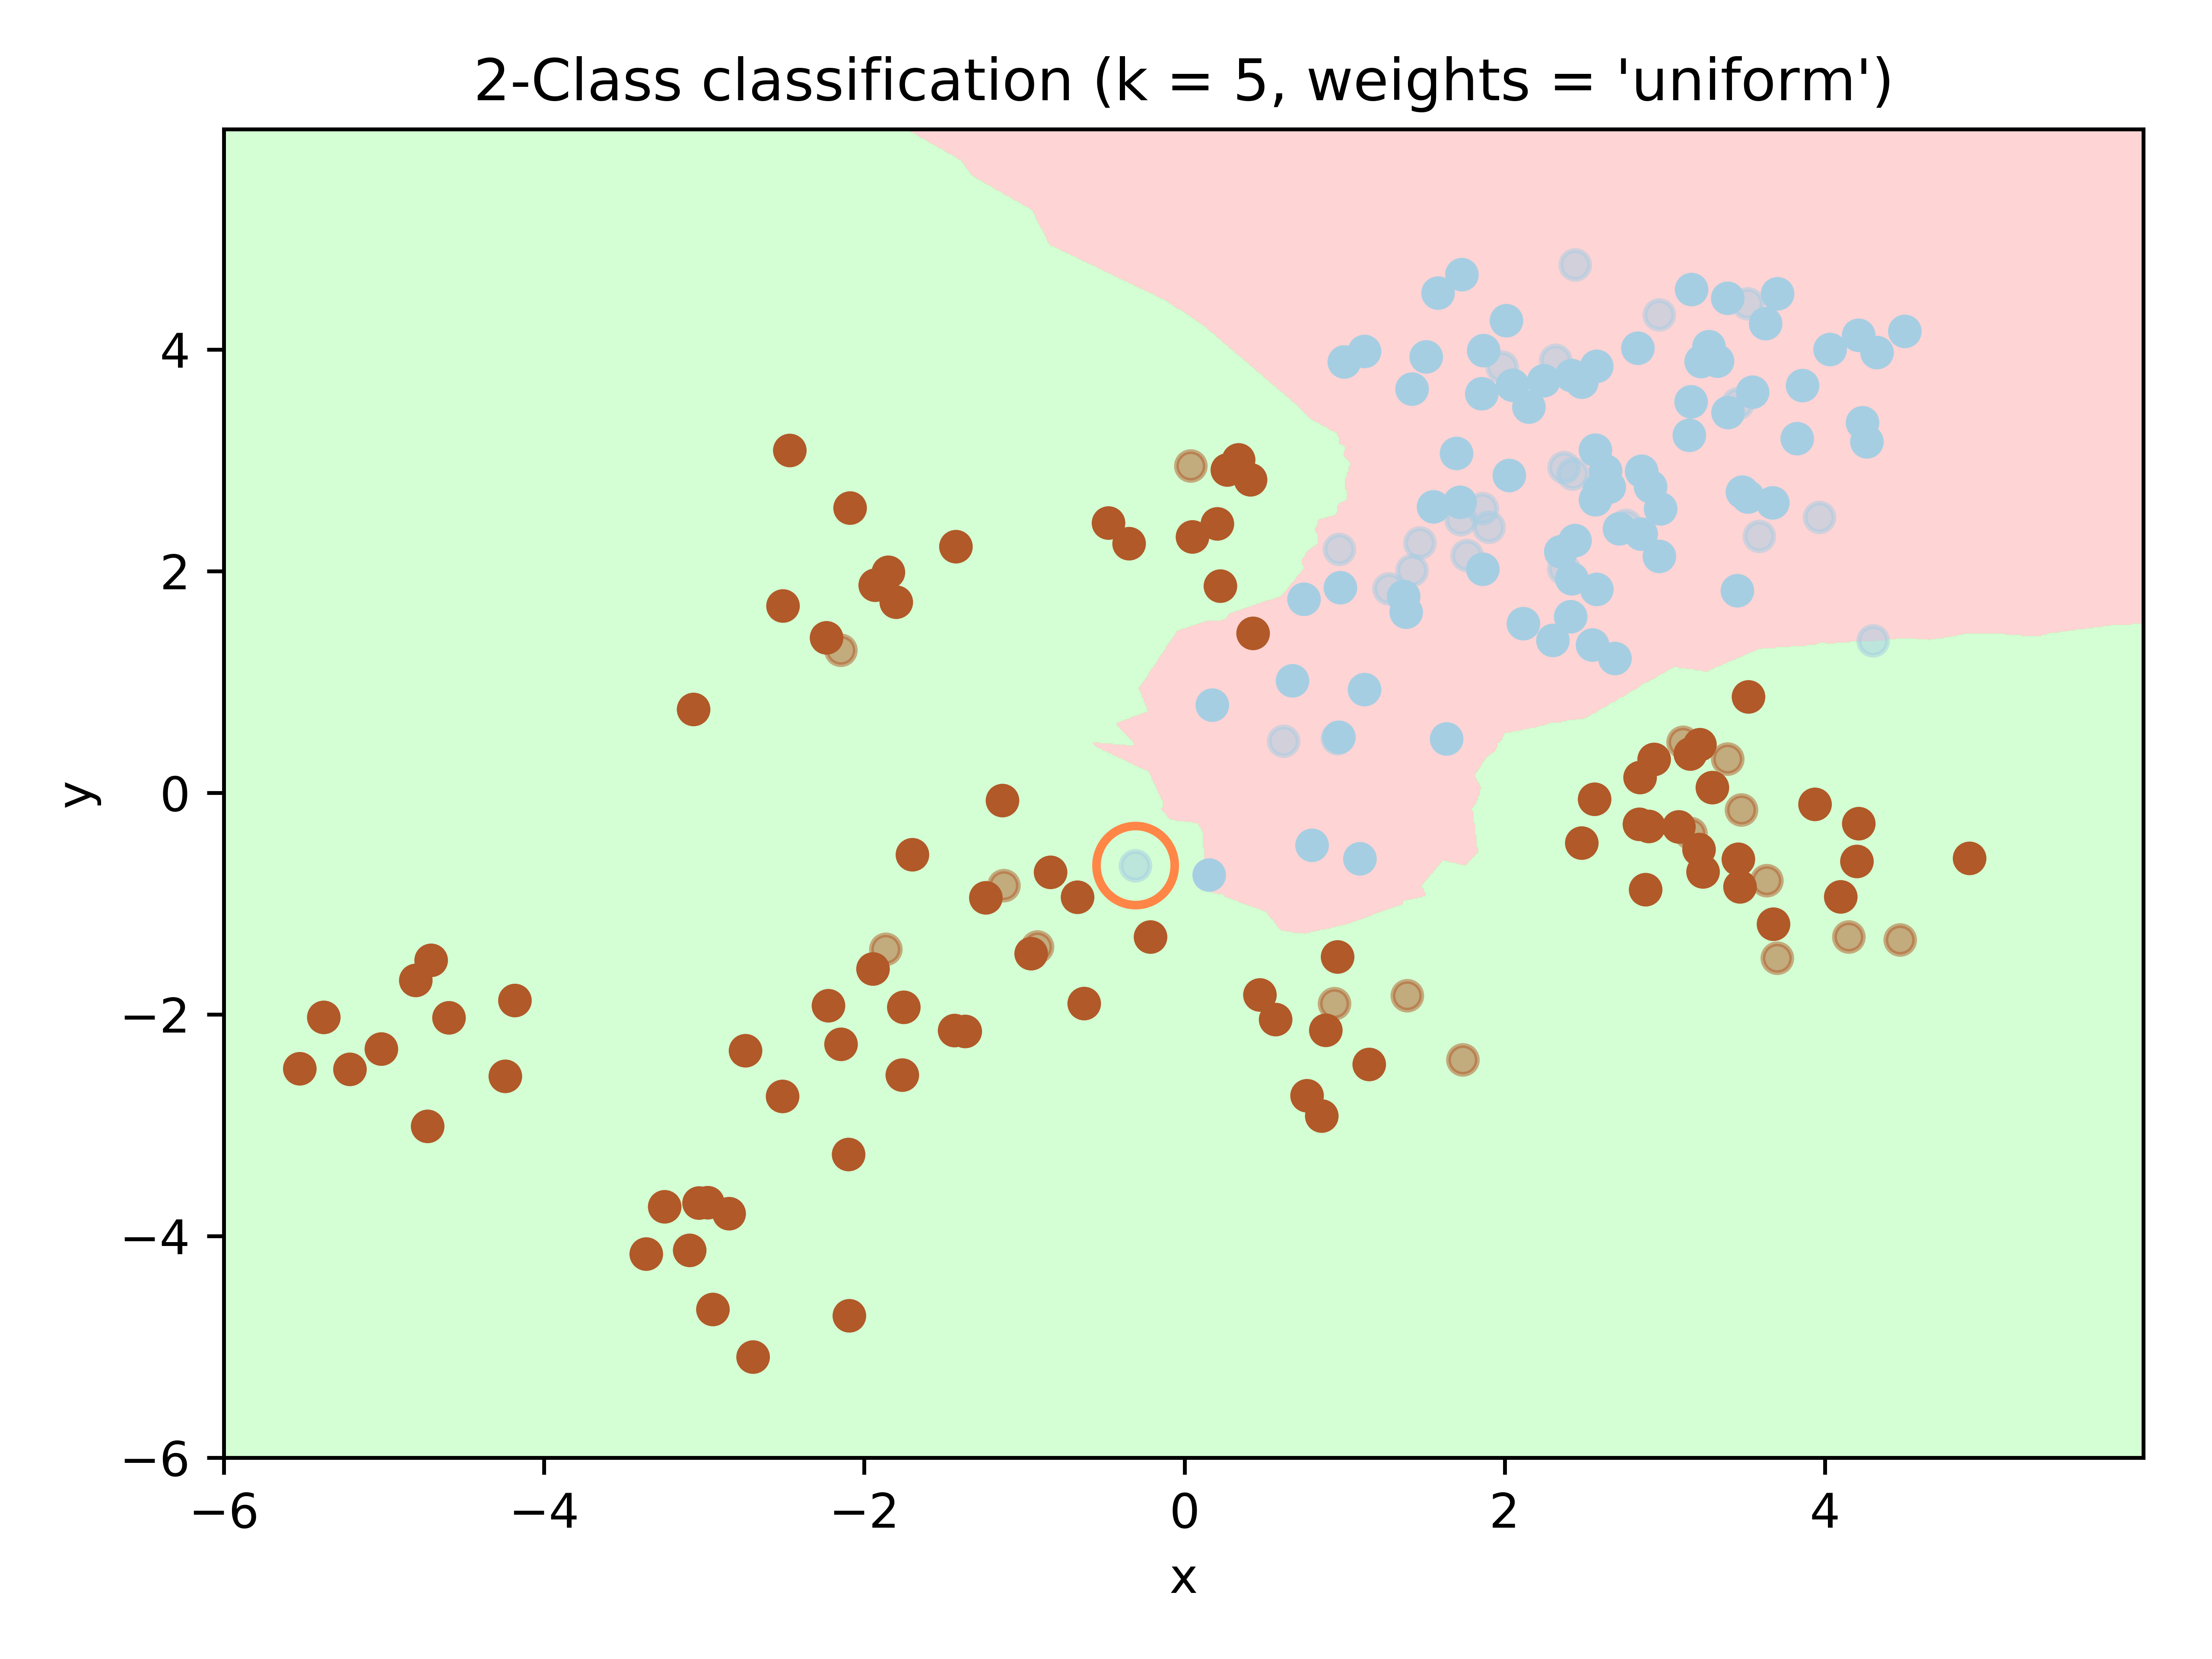
\includegraphics[width=0.6\linewidth]{img//fig7.png}
	\caption{KNN训练集+测试集分类结果}
\end{figure}

\hs 测试集的结果也十分明了,只有桔色框圈起来的是用训练的KNN在测试中误检的。\\


{\kaishu{\large KNN中$k$取值分析}}

\hs 这里利用的训练样本和测试集都选取的上面的实验一致,仅改变$k$的取值。

\hs $k=1$时,结果其precision、recall和f1-score如下:

\begin{table}[htbp]
	\caption{$k=1$时precision、recall和f1-score统计表}
	\centering
	\begin{tabular}{c|cccc}	
		& precision&recall&f1-score & support \\
		\hline
		1    &   0.96  &    1.00 &    0.98  &      22\\
		2    &   1.00    &  0.94   &   0.97    &    18 \\
		avg / total    &   0.98  &    0.97  &    0.97 &       40
	\end{tabular}	
\end{table}

\hs $k=1$其所有数据的分类结果(浅色为测试集,深色为训练集)如图4:

\begin{figure}[htbp]
	\centering
	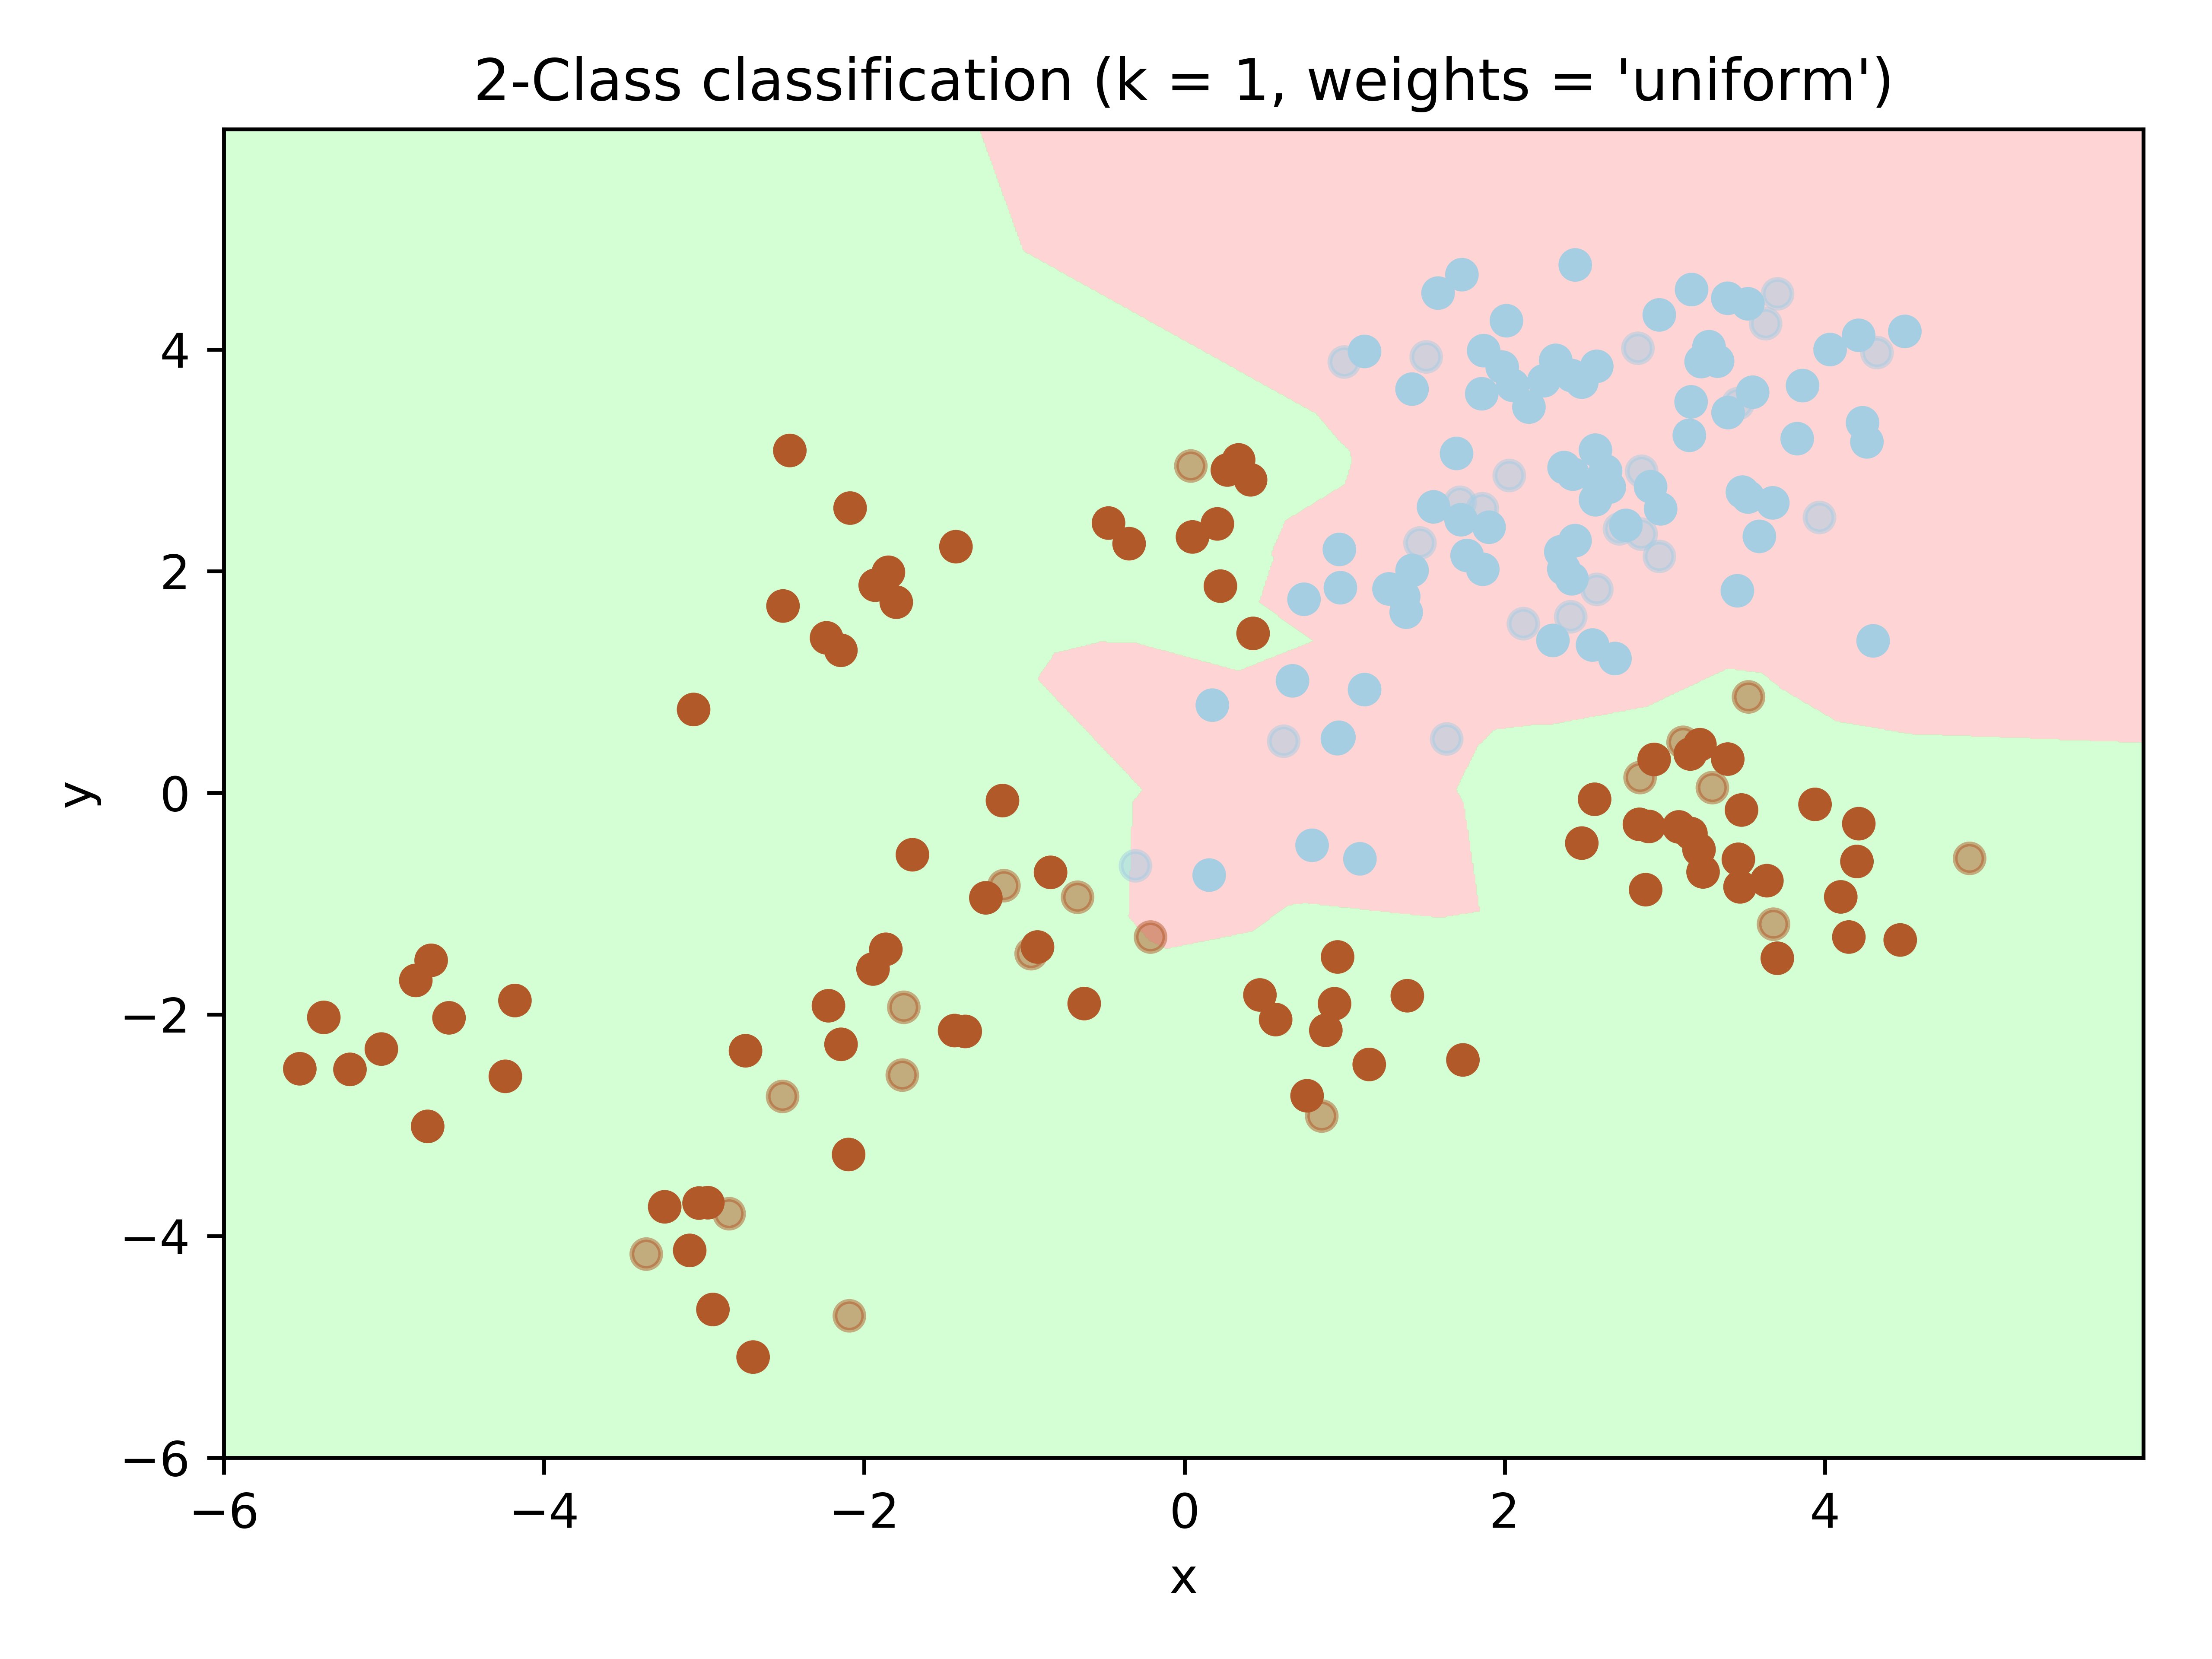
\includegraphics[width=0.6\linewidth]{img//fig2.png}
	\caption{$k=1$,KNN训练集+测试集分类结果}
\end{figure}


\hs $k=3$时,结果其precision、recall和f1-score如下:

\begin{table}[htbp]
	\caption{$k=3$时precision、recall和f1-score统计表}
	\centering
	\begin{tabular}{c|cccc}	
		& precision&recall&f1-score & support \\
		\hline
		1    &   1.00  &    0.95 &    0.98  &      22\\
		2    &   0.95    &  1.00   &   0.97    &    18 \\
		avg / total    &   0.98  &    0.97  &    0.98 &       40
	\end{tabular}	
\end{table}


\hs $k=3$其所有数据的分类结果(浅色为测试集,深色为训练集)如图5:

\begin{figure}[htbp]
	\centering
	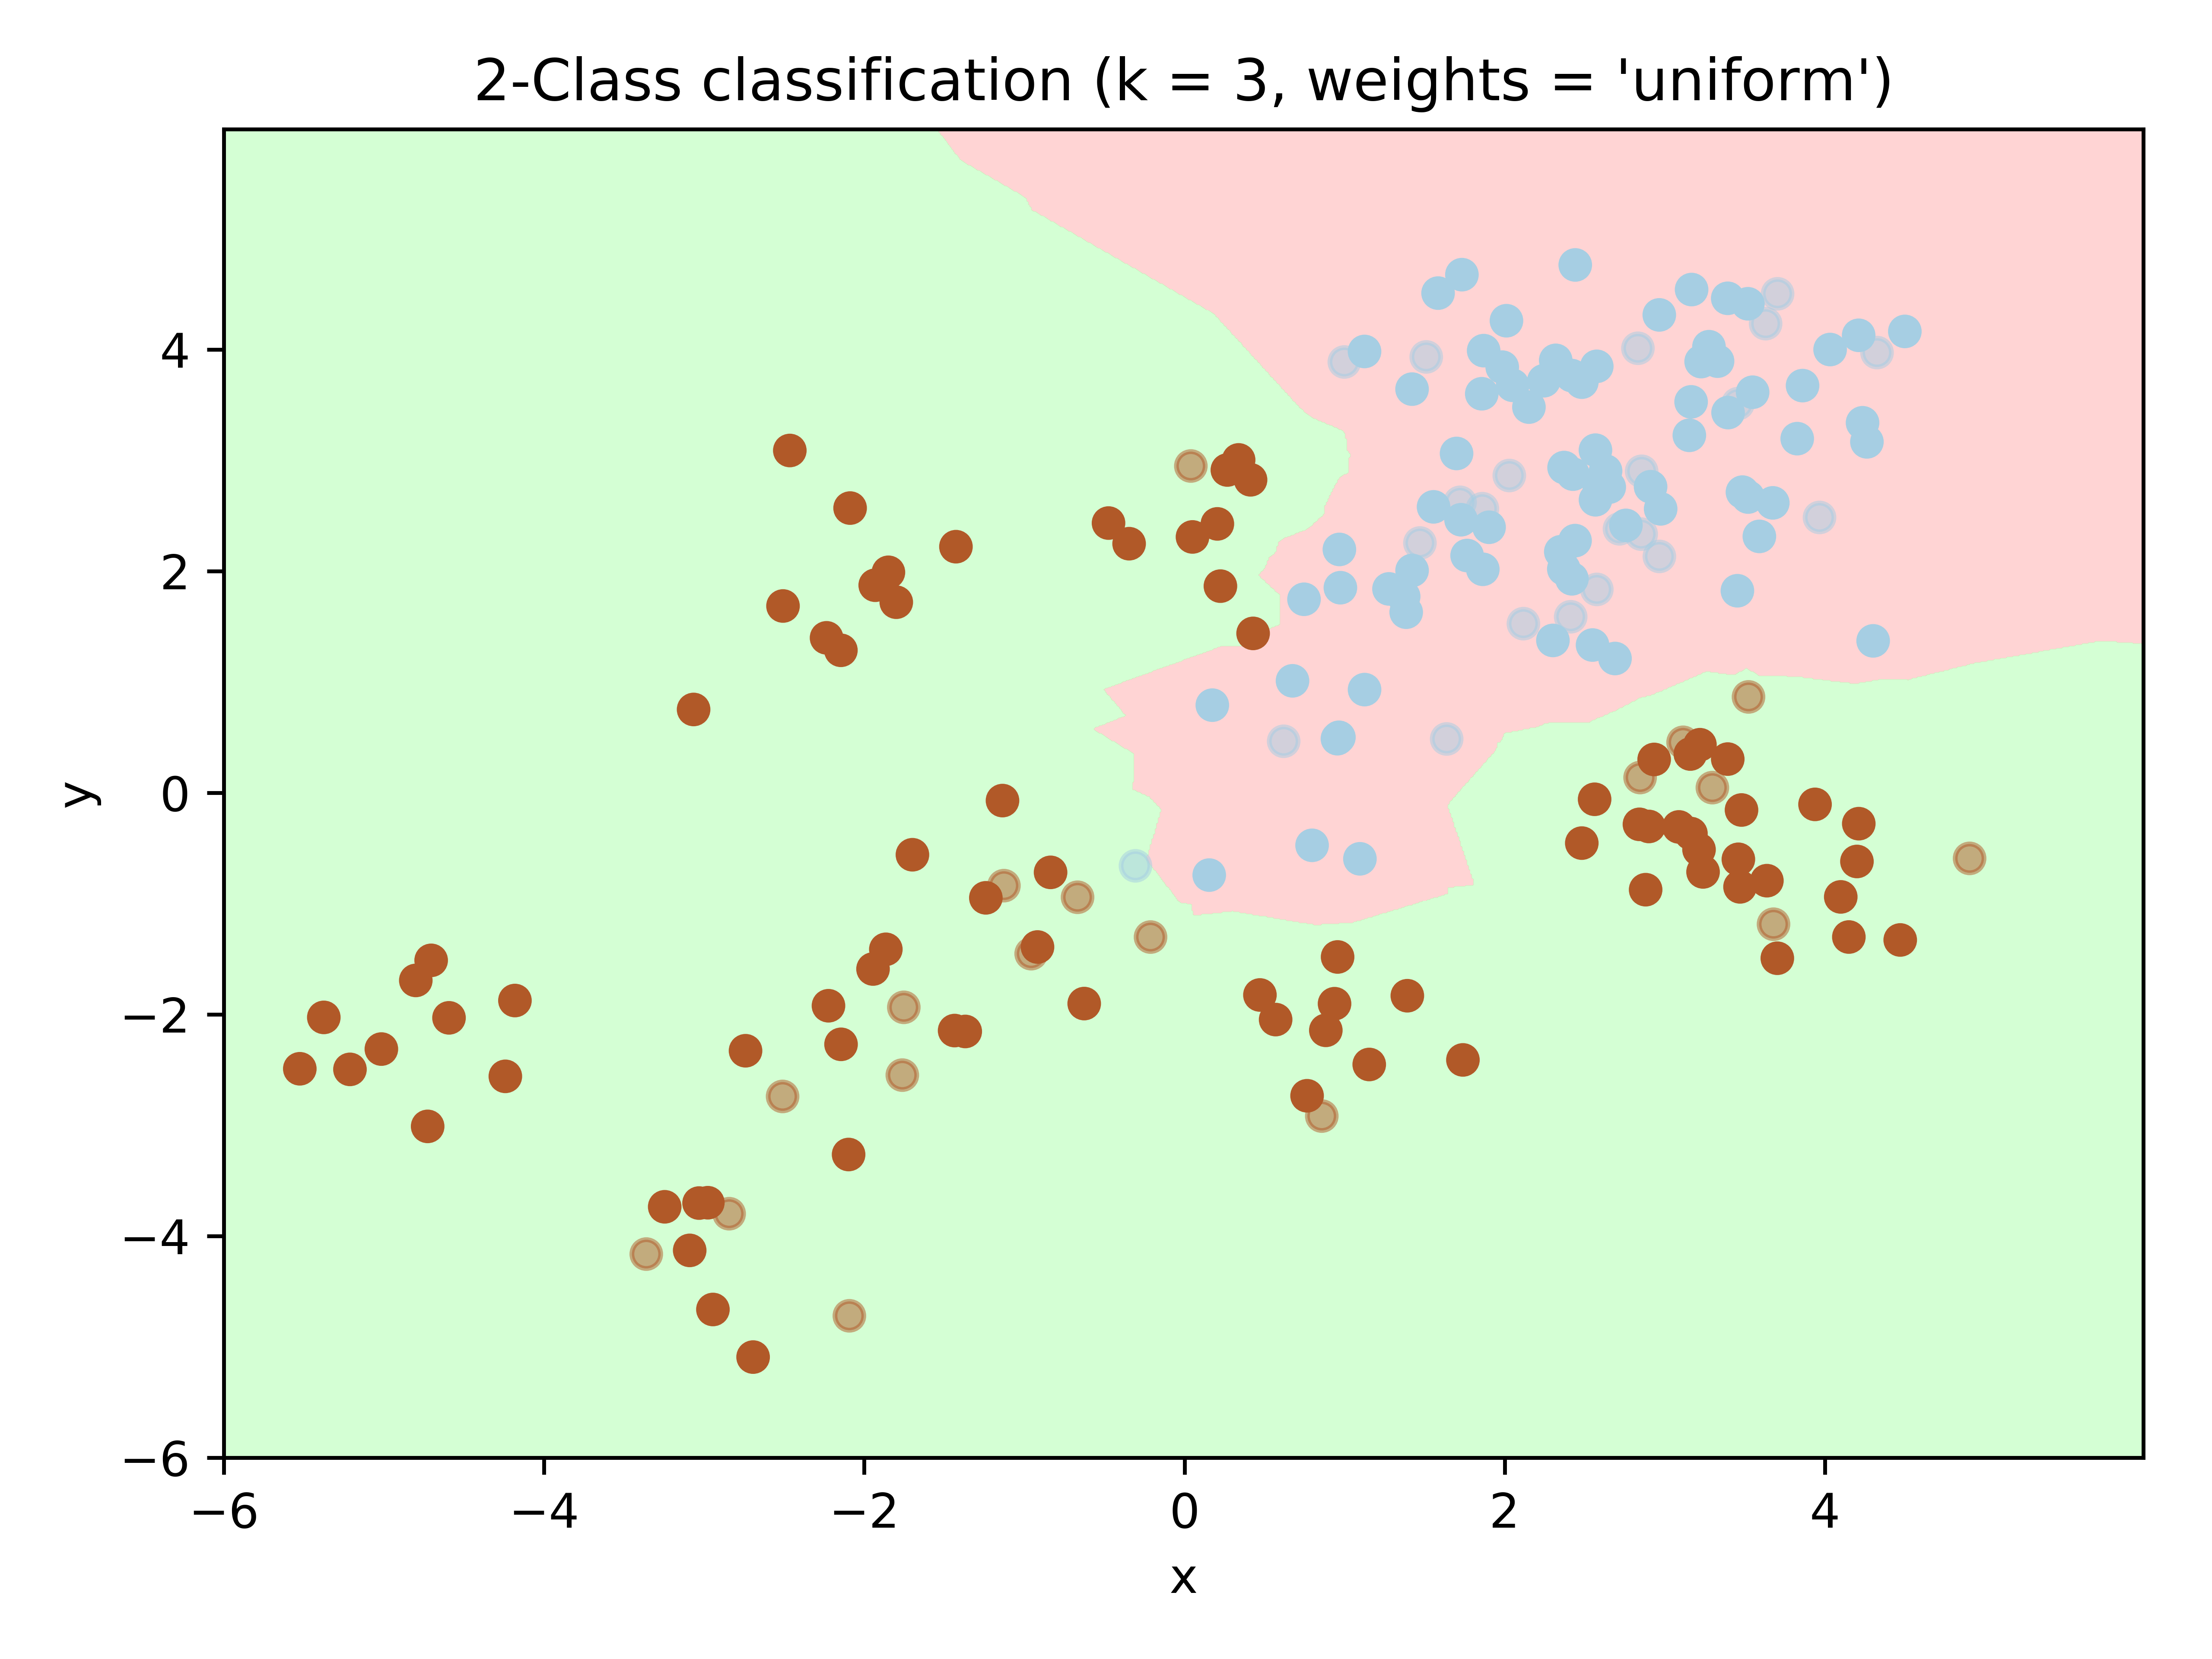
\includegraphics[width=0.6\linewidth]{img//fig3.png}
	\caption{$k=3$,KNN训练集+测试集分类结果}
\end{figure}


\hs $k=5$时,结果其precision、recall和f1-score如下表4:

\begin{table}[H]
	\caption{$k=5$时precision、recall和f1-score统计表}
	\centering
	\begin{tabular}{c|cccc}	
		& precision&recall&f1-score & support \\
		\hline
		1    &   1.00  &    0.95 &    0.98  &      22\\
		2    &   0.95    &  1.00   &   0.97    &    18 \\
		avg / total    &   0.98  &    0.97  &    0.98 &       40
	\end{tabular}	
\end{table}


\hs $k=5$其所有数据的分类结果(浅色为测试集,深色为训练集)如图5:

\begin{figure}[H]
	\centering
	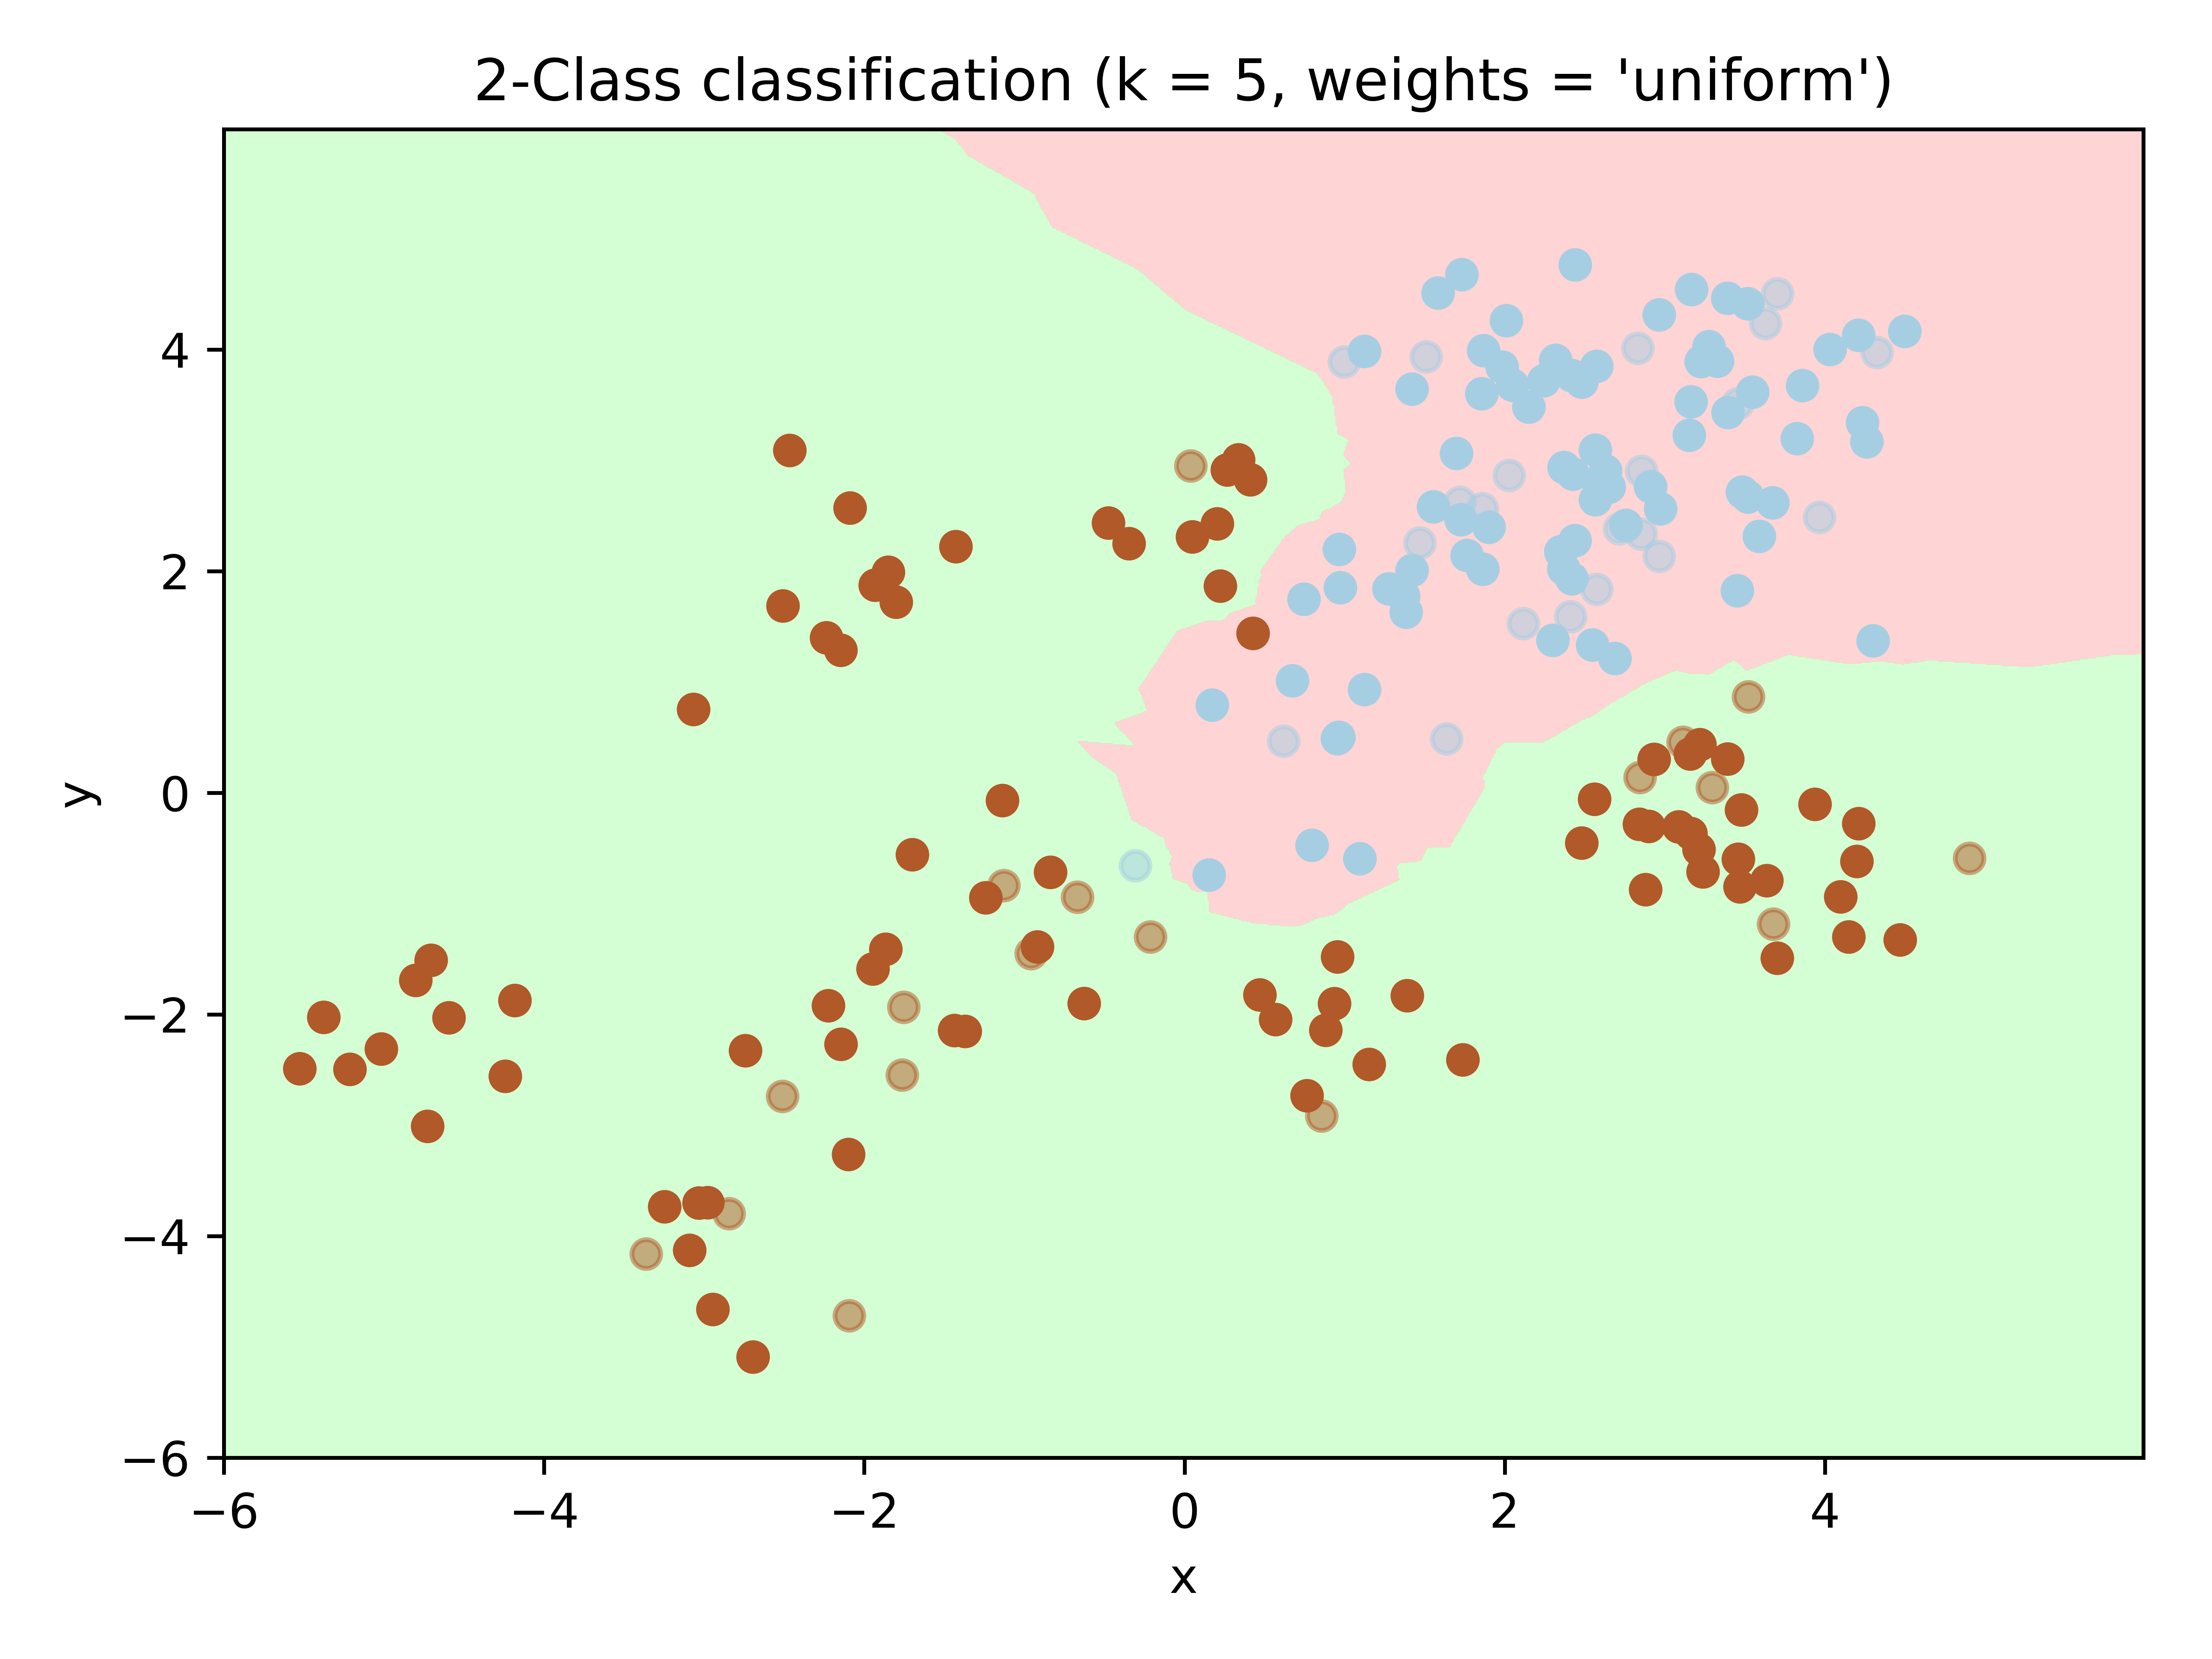
\includegraphics[width=0.6\linewidth]{img//fig4.png}
	\caption{$k=5$,KNN训练集+测试集分类结果}
\end{figure}

\hs  将上述结果进行对比分析,不难发现随着$k$的不断增加,分界面变得越来越平坦,也使得precision、recall和f1-score相比于最近邻都有所提升,这是符合产常识的。根据欧卡姆剃刀准则,这些分界面应该尽量显得“简单”,少一些“曲折”。\\


{\kaishu{\large KNN中$k=5$,K分析 }}

\hs  上面的测试都将$k$个最近邻一视同仁,并没有分配权重,或者说权重都一致。这样的设置对于某些情况并不适合,比如数据点符合高斯分布,这需要我们按照一定规则分配周围一些点的权重。最简单的想法就是按照距离分配权重,当然这时候“距离”也可以是多种多样,如欧式距离,曼哈顿距离,切比雪夫距离, 闵可夫斯基距离等。这里我选择最常见的欧氏距离作为权重分配的规则,即离测试点越近的点分配的权重越多。

\hs 训练和测试的样本集和上面的实验一致,且令$k=5$,仅改变weights,由原来的“uniform“,改为”distance“。得到下面图7和图8的对比结果:



\begin{figure}[htbp]
	\begin{minipage}[b]{.5\linewidth}
		\centering
		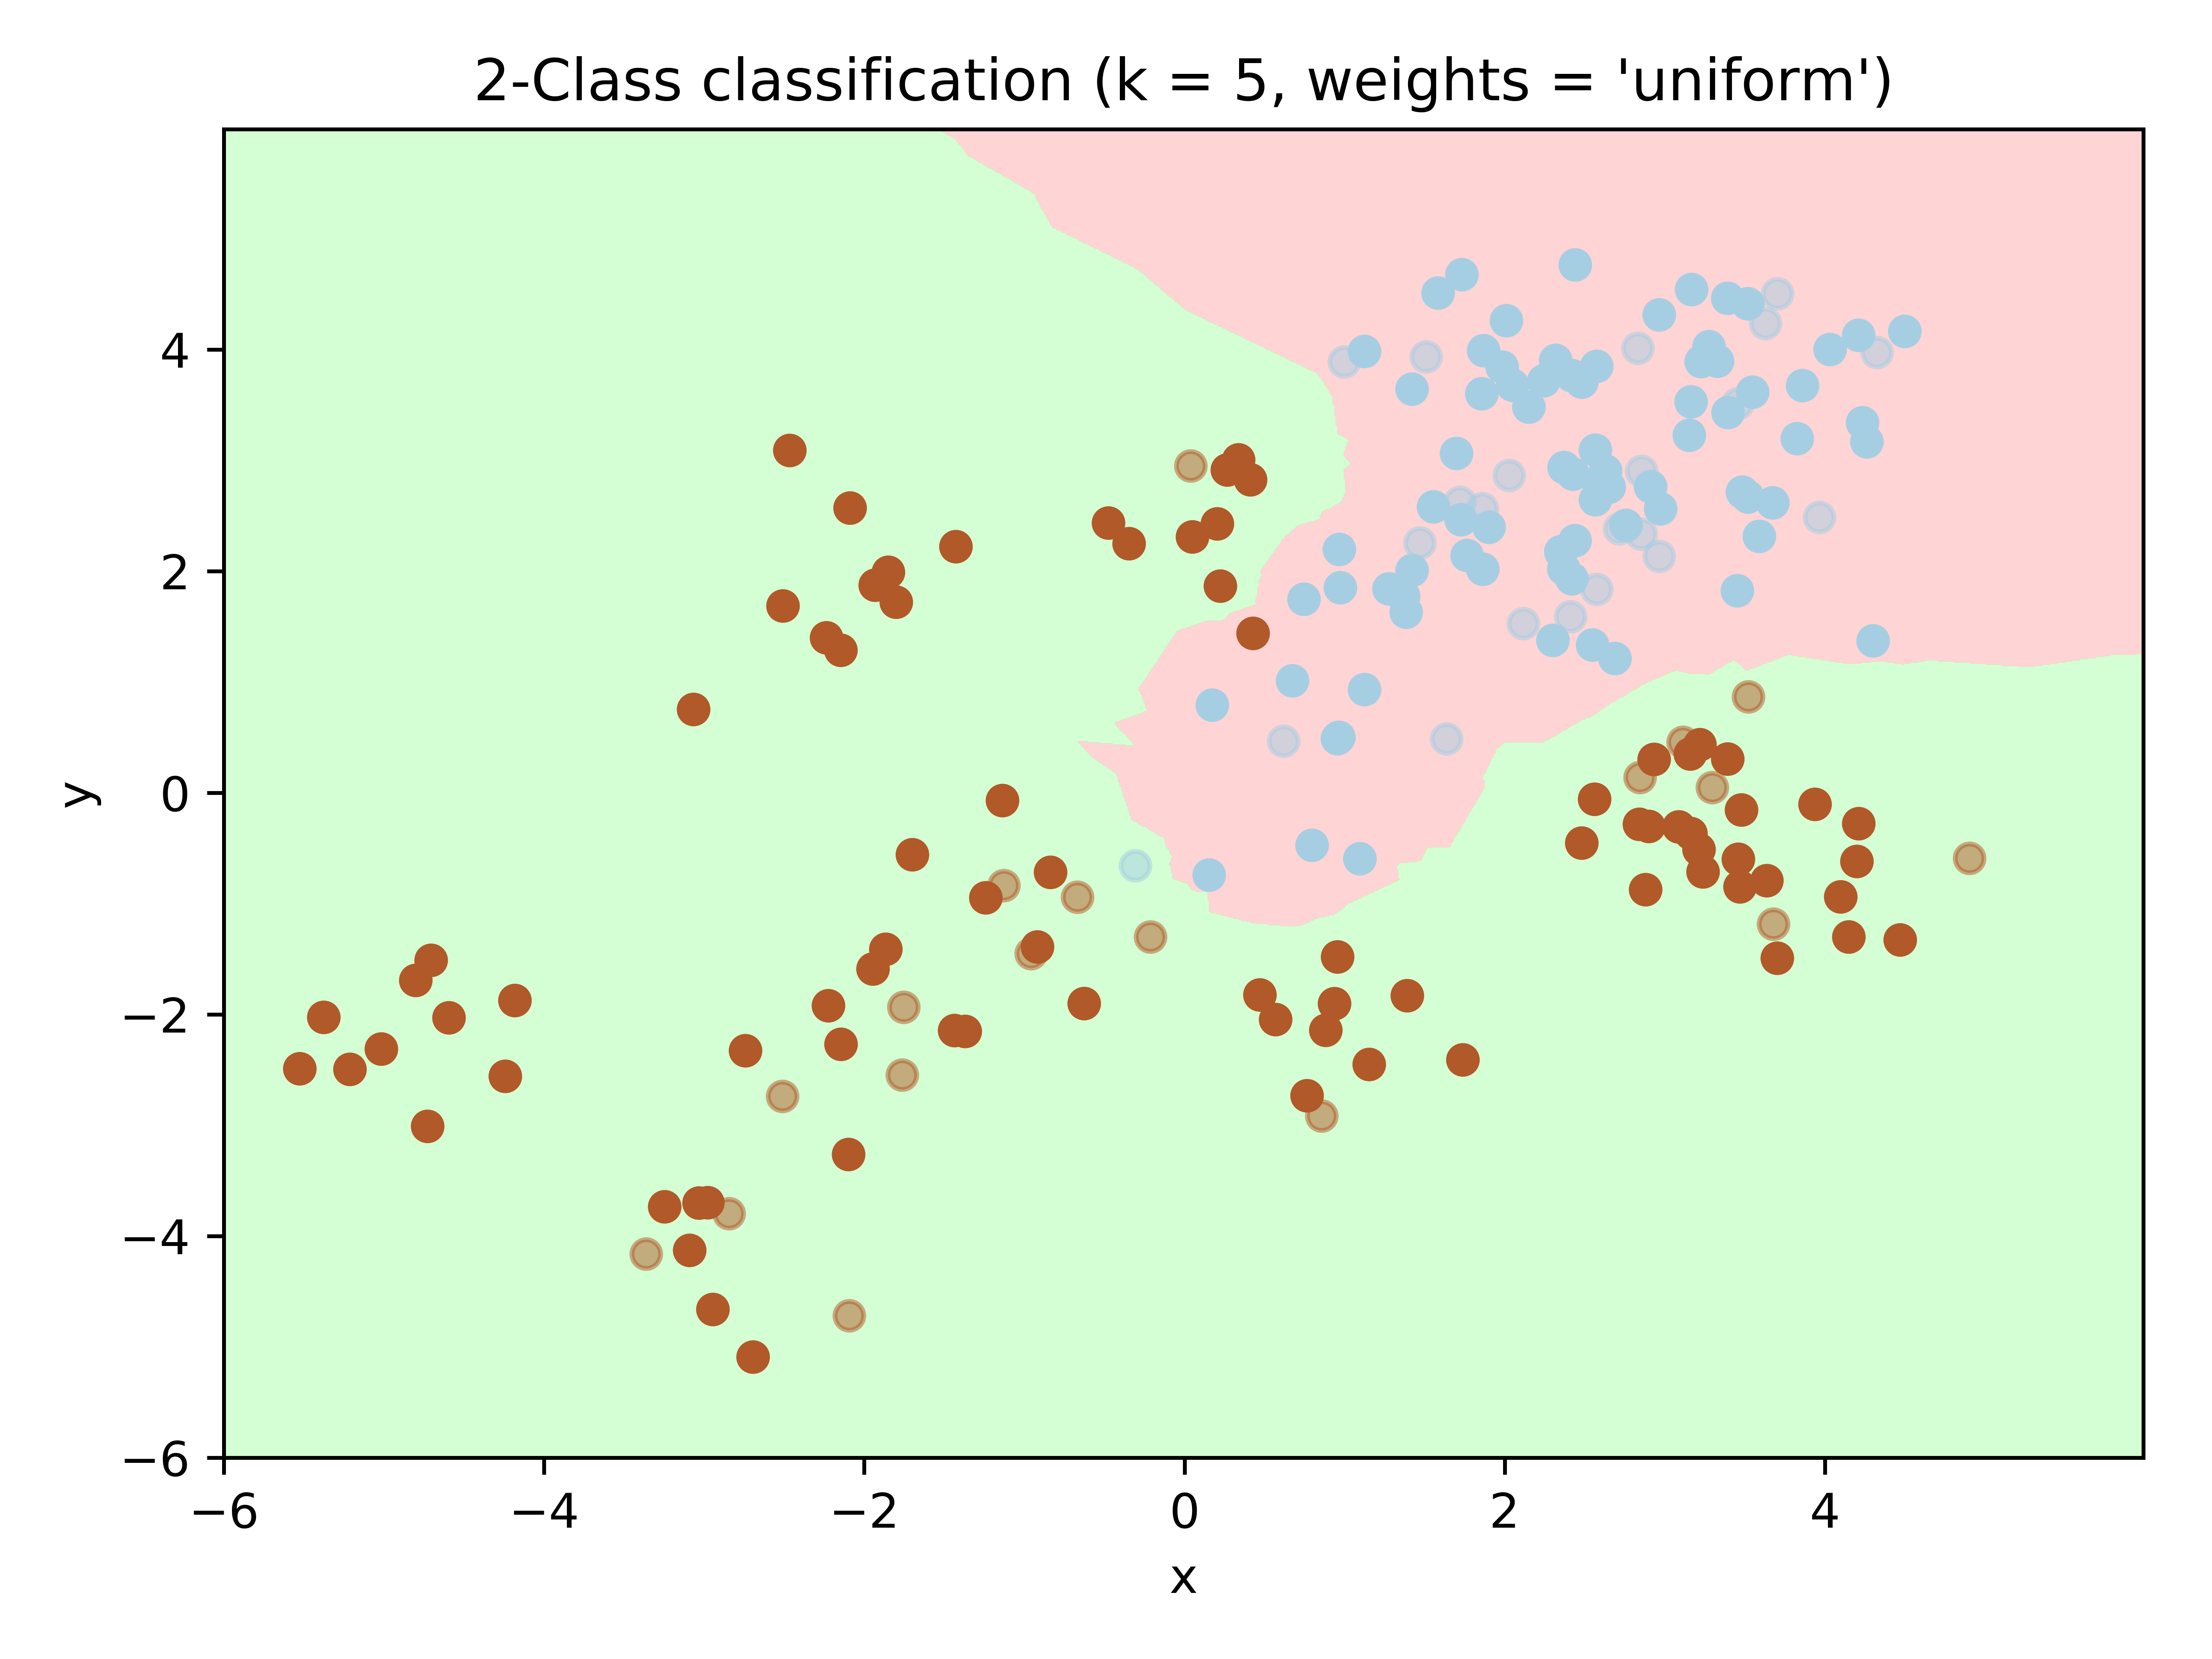
\includegraphics[width=6.5cm]{img//fig4.png}
		\caption{weights=uniform}
	\end{minipage}%
	\begin{minipage}[b]{.5\linewidth}
	\centering
	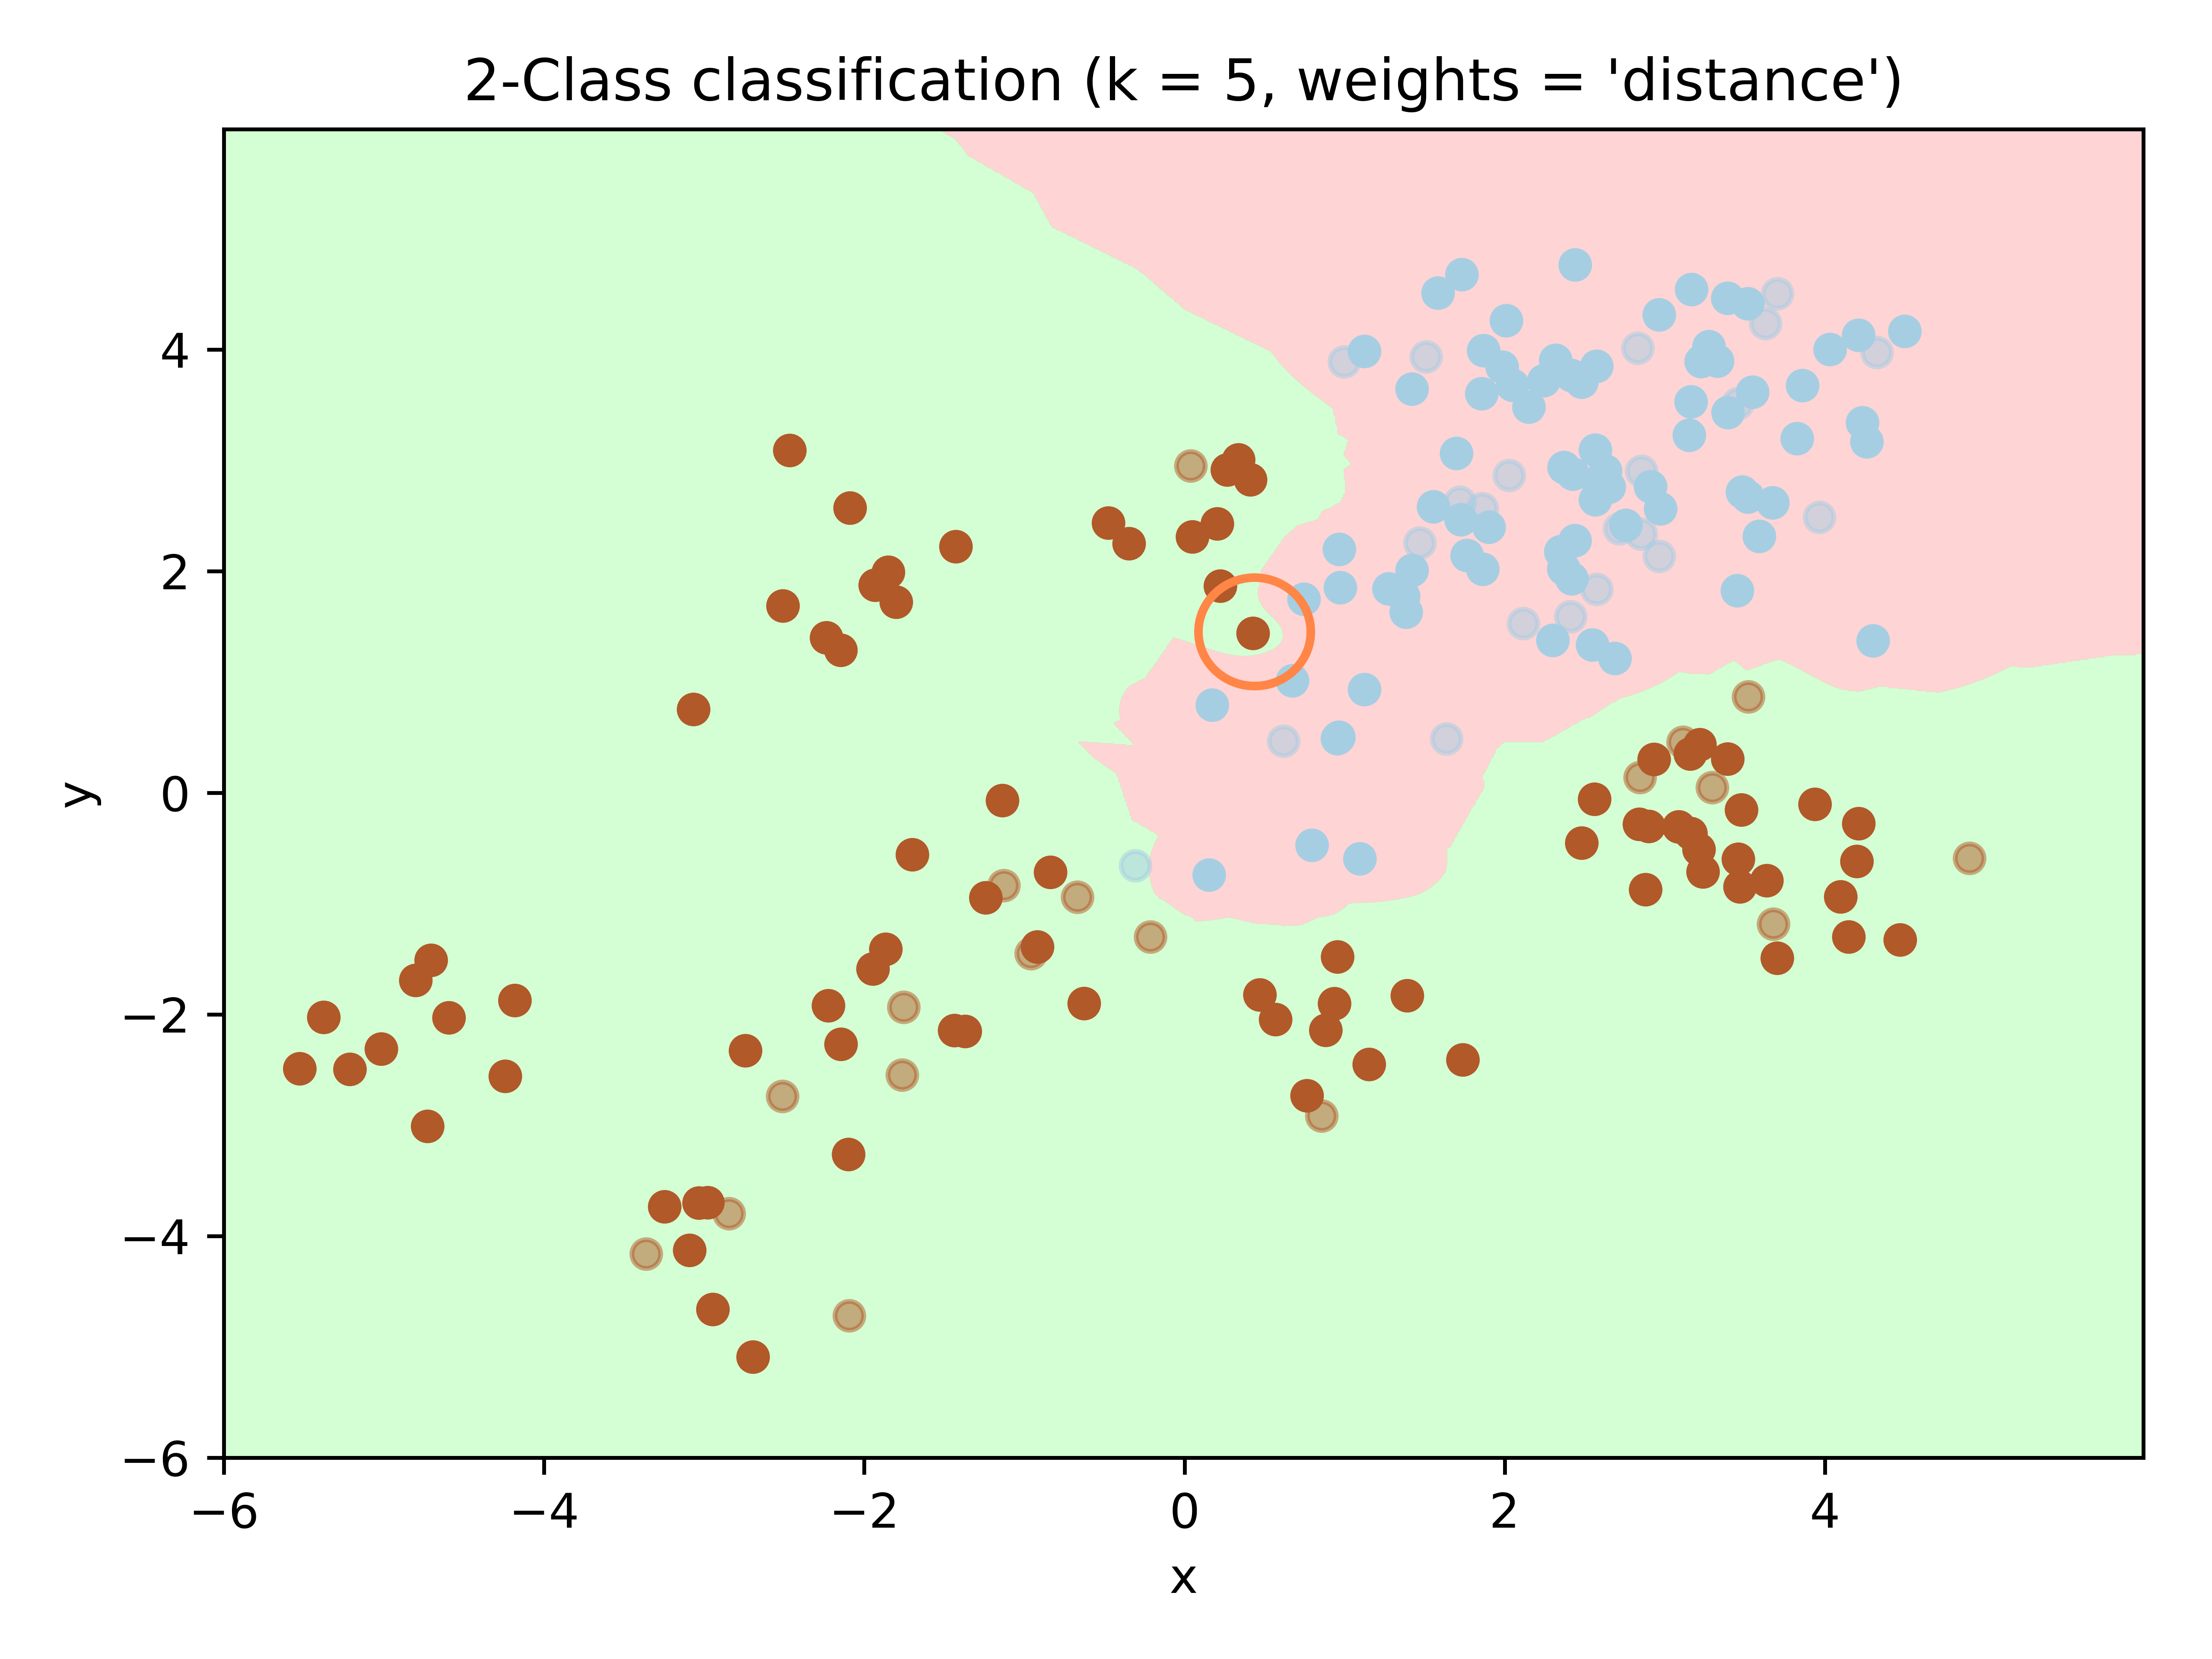
\includegraphics[width=6.5cm]{img//fig10.png}
	\caption{weights=distance}
\end{minipage}%
\end{figure}


\hs 对上述两者,发现两者相差并不多,只有在局部的细节部分有不一样的部分。特别注意的当权重设置为distance时,图8中那个特别的点就被训练出来了,究其原因,根据距离分配权重的方法,对于自身点,因为距离为0,定然其权重就很大,因此该点被训练出来了。而在平均权重的方案,该点的被其他周围的点给均化了,而从训练不出来该点。\\


{\kaishu{\large k近邻高效算法实现}}

\hs 近邻算法当样本数目较多时,才能取得比较好的性能,但是,新样本计算距离然后通过排序的法找出$k$个最近邻的点,当样本数目较多的时候,其计算量会非常大,这里使用kd-tree法和普通的蛮力算法进行比较。

\hs KD树建树采用的是从m个样本的n维特征中,分别计算n个特征的取值的方差,用方差最大的第k维特征$n_k$来作为根节点。对于这个特征,选择特征$n_k$的取值的中位数$n_{kv}$对应的样本作为划分点,对于所有第k维特征的取值小于$n_{kv}$的样本,划入左子树,对于第k维特征的取值大于等于$n_{kv}$的样本,划入右子树,对于左子树和右子树,采用和刚才同样的办法来找方差最大的特征来做更节点,递归的生成KD树。

\hs 具体流程如下图:

\begin{figure}[htbp]
	\centering
	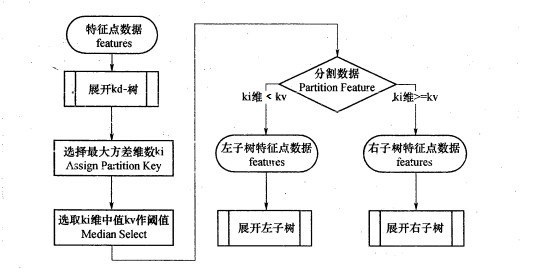
\includegraphics[width=0.6\linewidth]{img//fig9}
	\caption{KD树流程图}
\end{figure}

由于数据样本还是相对偏少,因此在这个实验中,KD树的优势并没有体现出来。下面是统计时间表,单位为秒(s)。

\begin{table}[htbp]
	\caption{$k=5$时蛮力算法和kd-tree比较统计表}
	\centering
	\begin{tabular}{c|ccc}	
	train集合占比	& 0.8 & 0.9 & 0.99 \\
		\hline
	蛮力    &   0.000346  &    0.000431  &  0.000433 \\
	kd-tree    &   0.000512    &  0.000586  & 0.000538 \\
	\end{tabular}	
\end{table}

为了对KD进行实验,随机生成了1000000个样本进行测试,样本分布如下:

\begin{figure}[htbp]
	\centering
	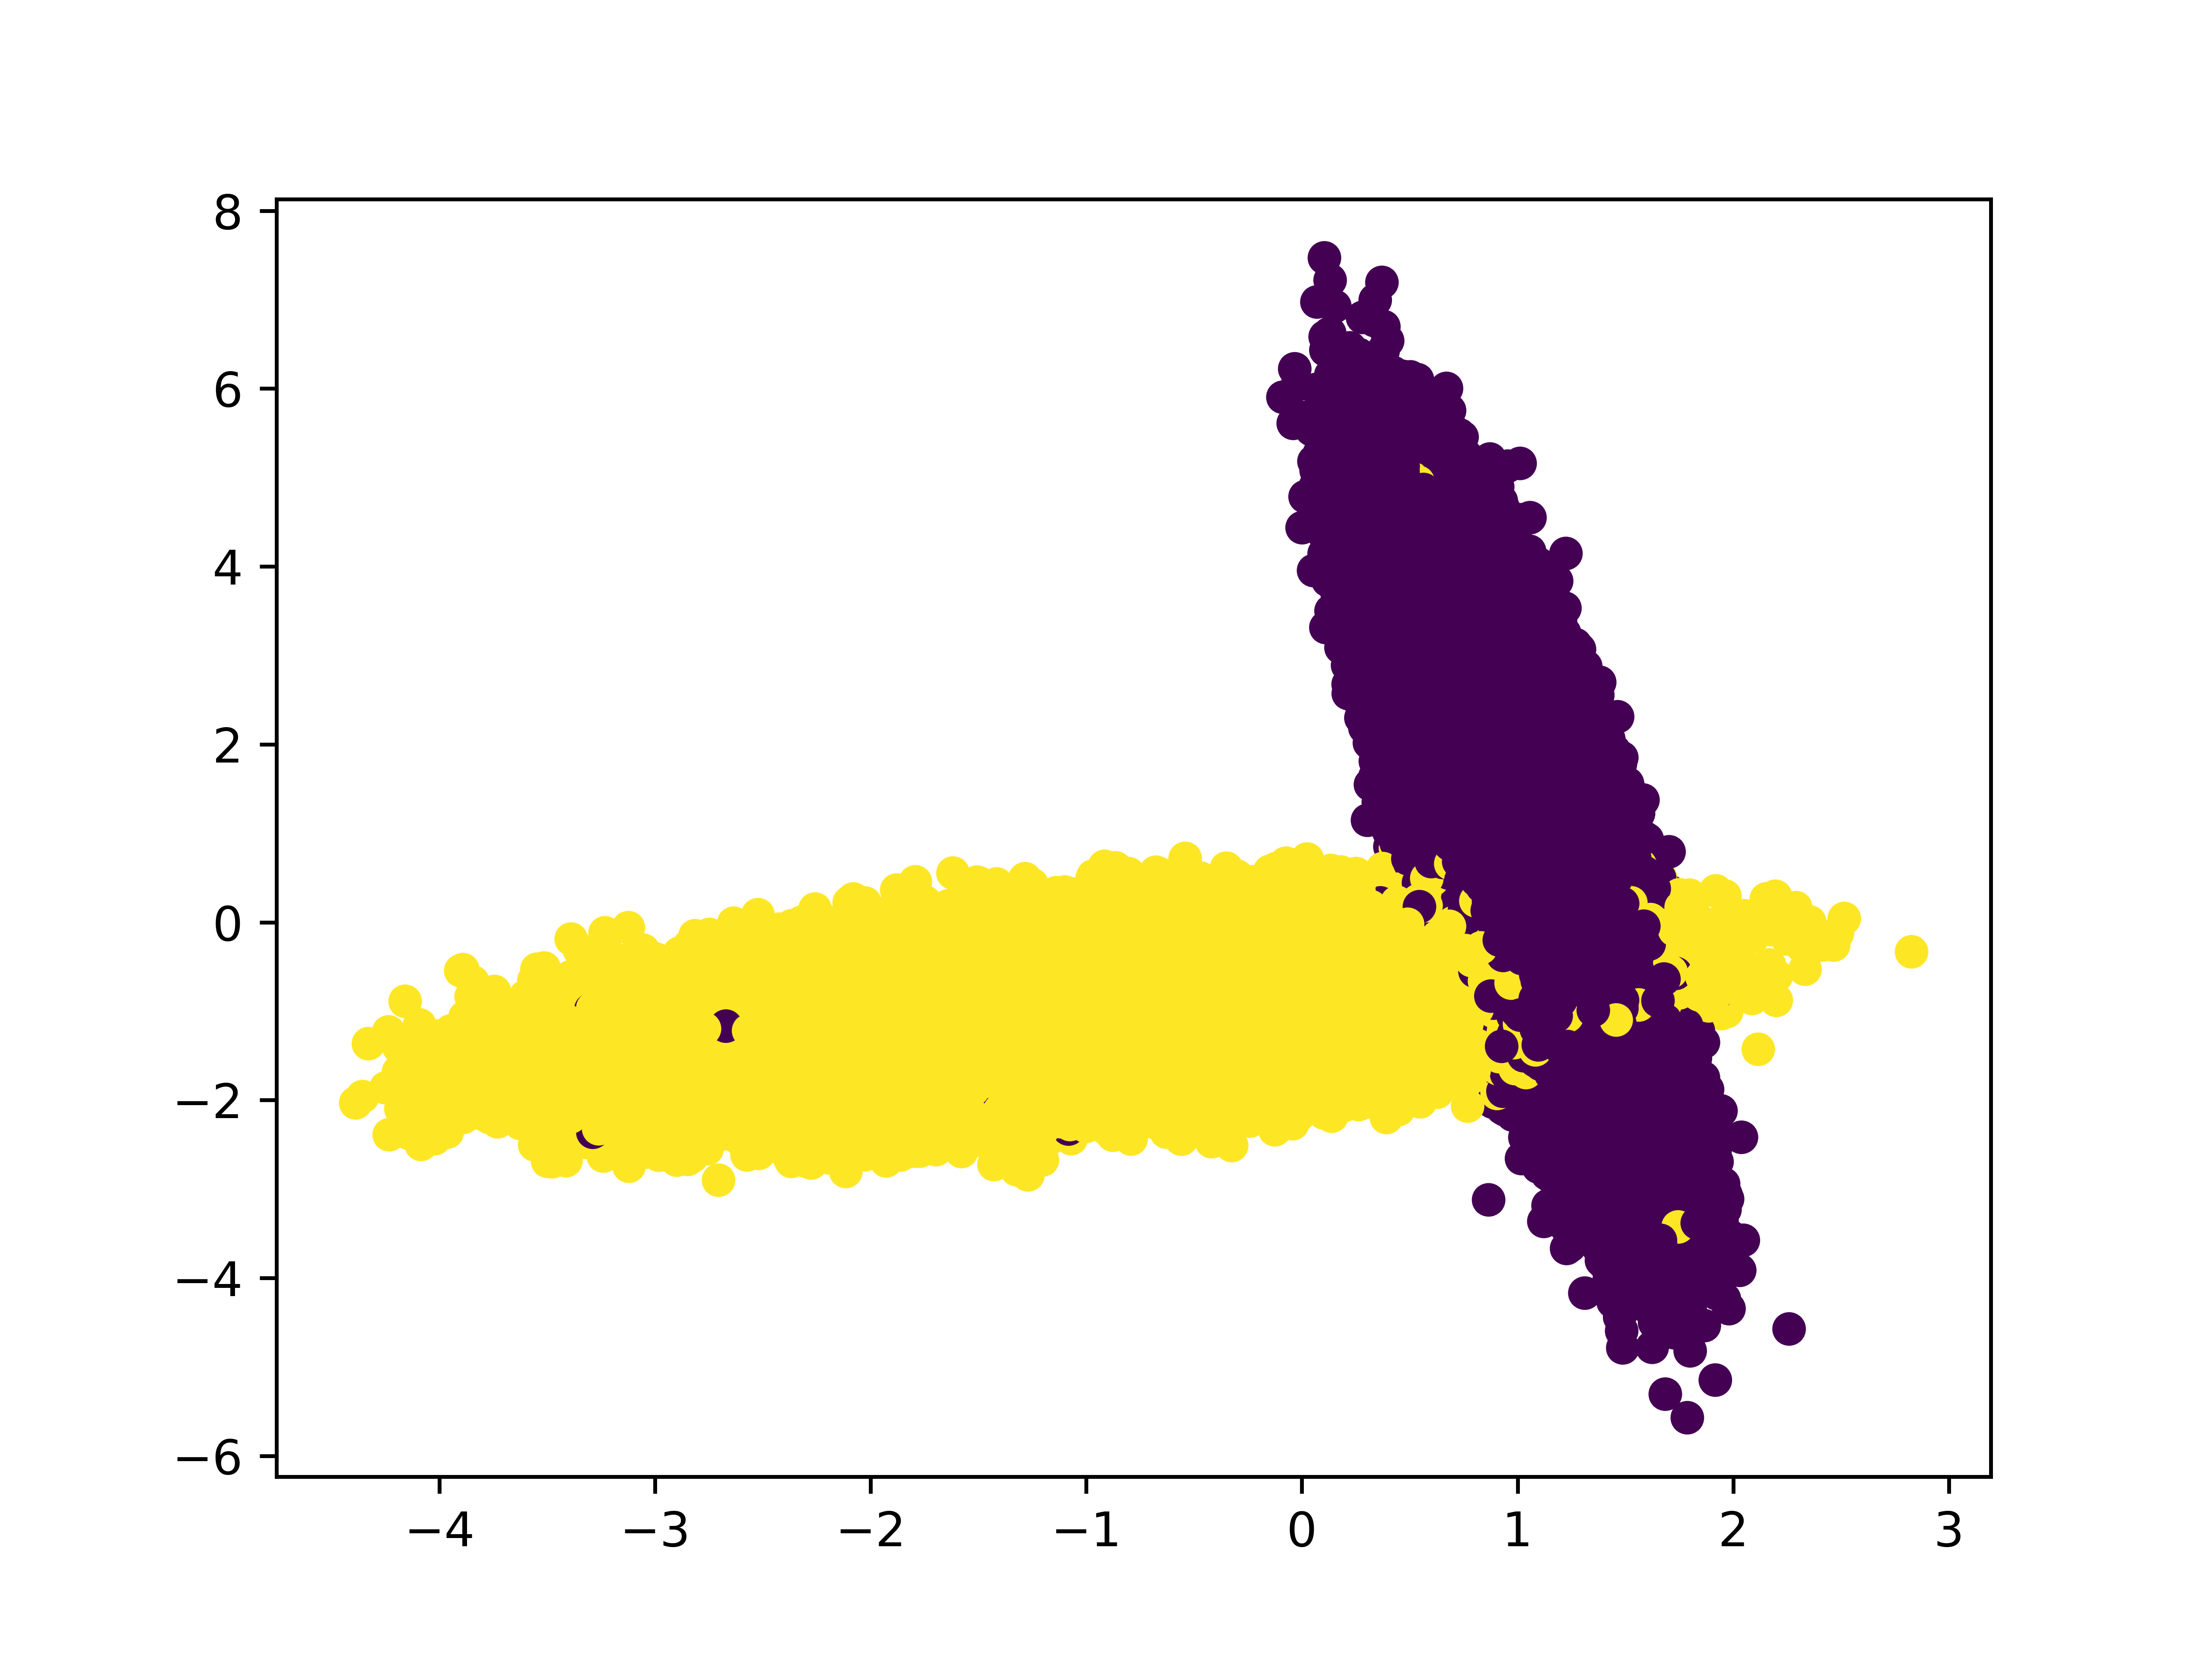
\includegraphics[width=0.6\linewidth]{img//fig8}
	\caption{1000000个样本分布}
\end{figure}

\hs 分别利用蛮力和kd-tree来实现,样本训练的时间分别为:1.881834s和0.130337s,在较大的数量的时候,kd-tree确实相比于蛮力更快。

\newpage

\section{Problem Two}
{\kaishu{\large Fisher判别}}

\hs 对下列两种情况,求采用Fisher判别准则 时的投影向量W和分类界面,并作图。

\begin{align*}
\omega_1 &= \{(2,0)  ,(2,2)  ,(2,4) ,(3,3)\}\\
\omega_2 &= \{(0, 3), (-2, 2), (-1, -1), (1, -2), (3, -1)\}
\end{align*}

\begin{align*}
\omega_1 &= \{(1, 1), (2, 0), (2, 1), (0, 2), (1, 3)\}\\
\omega_2 &= \{(-1, 2), (0, 0), (-1, 0), (-1, -1), (0, -2)\}
\end{align*}

\hs 本质上Fisher线性判别的思想就是,选择投影方向,使得投影后两类相隔尽可能的远,而同时,每一类内部的样本又尽可能的聚集。

\subsection{Fisher算法实验结果分析}
{\kaishu{\large $w_0$的确定}}

\hs $w$的最优投影方向为:
\begin{equation*}
w^* = S_w^{-1}(m_1-m_2)
\end{equation*}

值得注意的是,本身Fisher准则的最优解本身只是给出了一个投影方向,并没有给出分类面。要得到分类面,需要在投影后的方向(一维空间)上确定一个分类阈值$w_0$。一般不过考先验概率,则一般采用如下的$w_0$:

\begin{equation*}
w_0 = -\frac{1}{2}(\widetilde{m}_1+\widetilde{m}_2)
\end{equation*}

{\kaishu{\large 第一种情形}}

\hs 经过计算得到的结果:$w=(0.19241083,~0.12644141),~w_0=-0.390593993028$,其分界面函数就为:$0.1924x+0.1264y-0.3906=0$。$w$和分界面如下图11所示:
\begin{figure}[htbp]
	\centering
	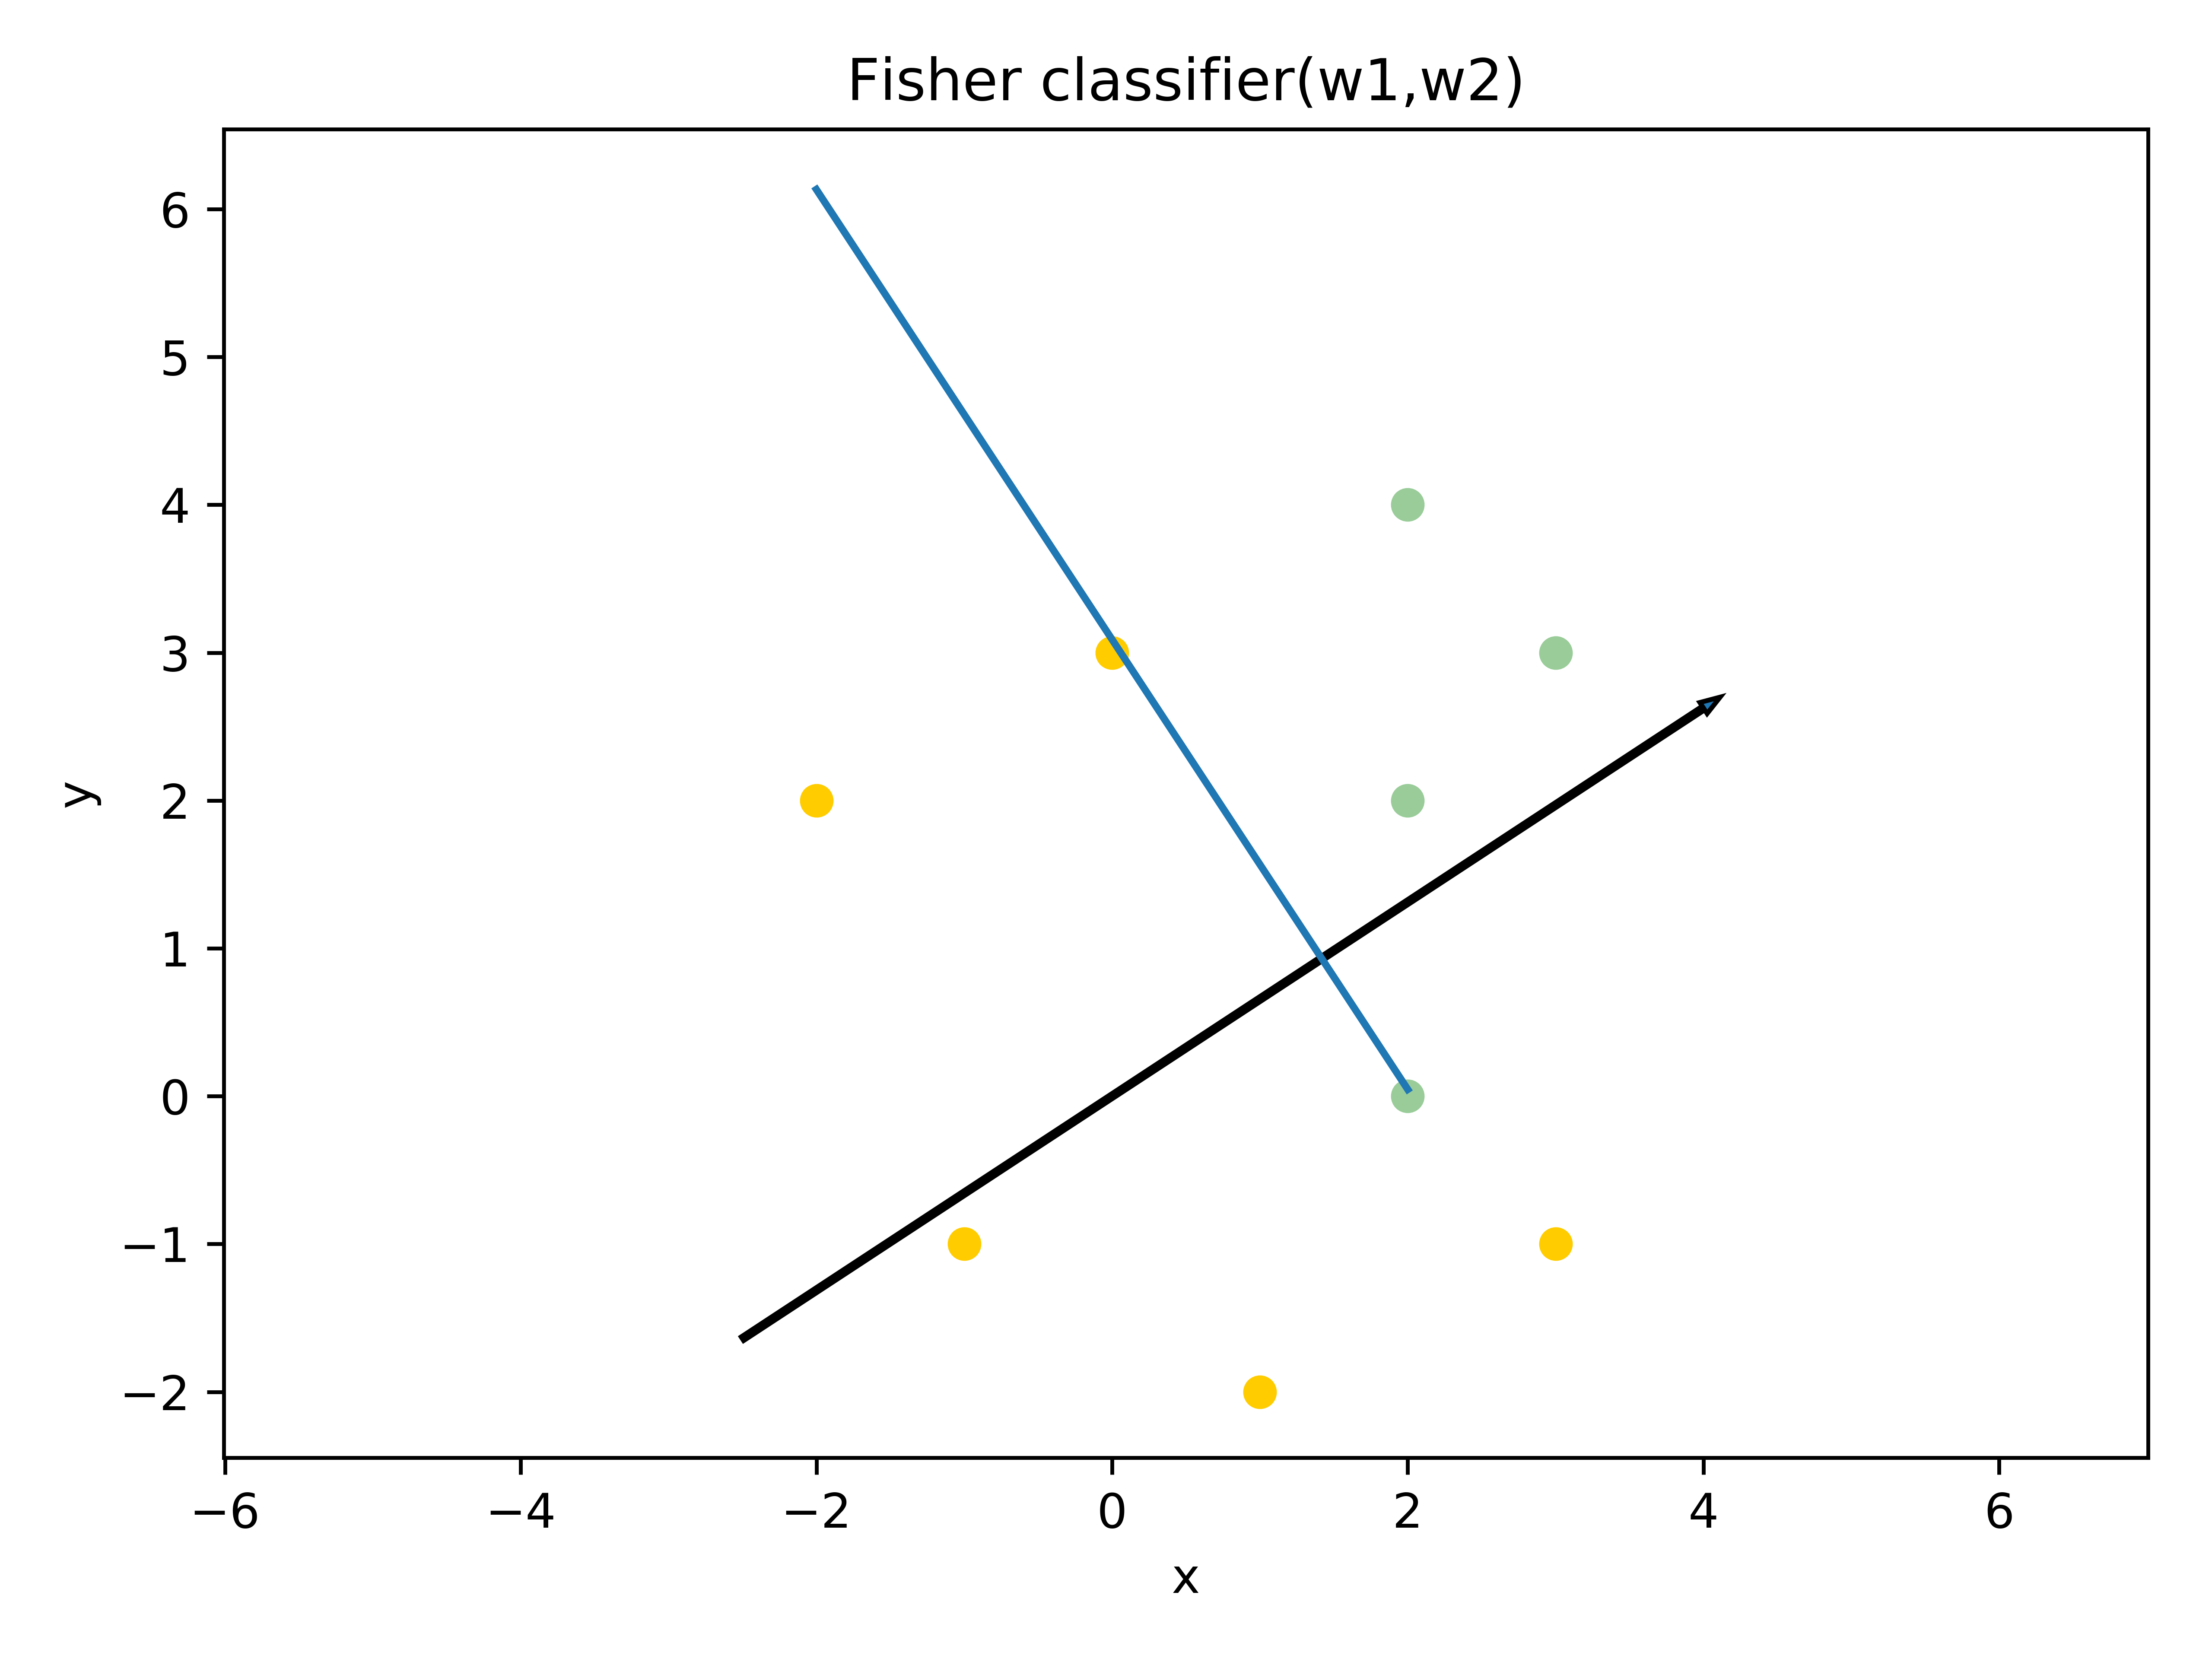
\includegraphics[width=0.6\linewidth]{img//fig12}
	\caption{Fisher判决的$w$和分界面}
\end{figure}


{\kaishu{\large 第二种情形}}

\hs 经过计算得到的结果:$w=(0.79,0.34),~w_0=-0.441$,其分界面函数就为:$0.79x+0.34y-0.441 =0 $。$w$和分界面如下图12所示:
\begin{figure}[htbp]
	\centering
	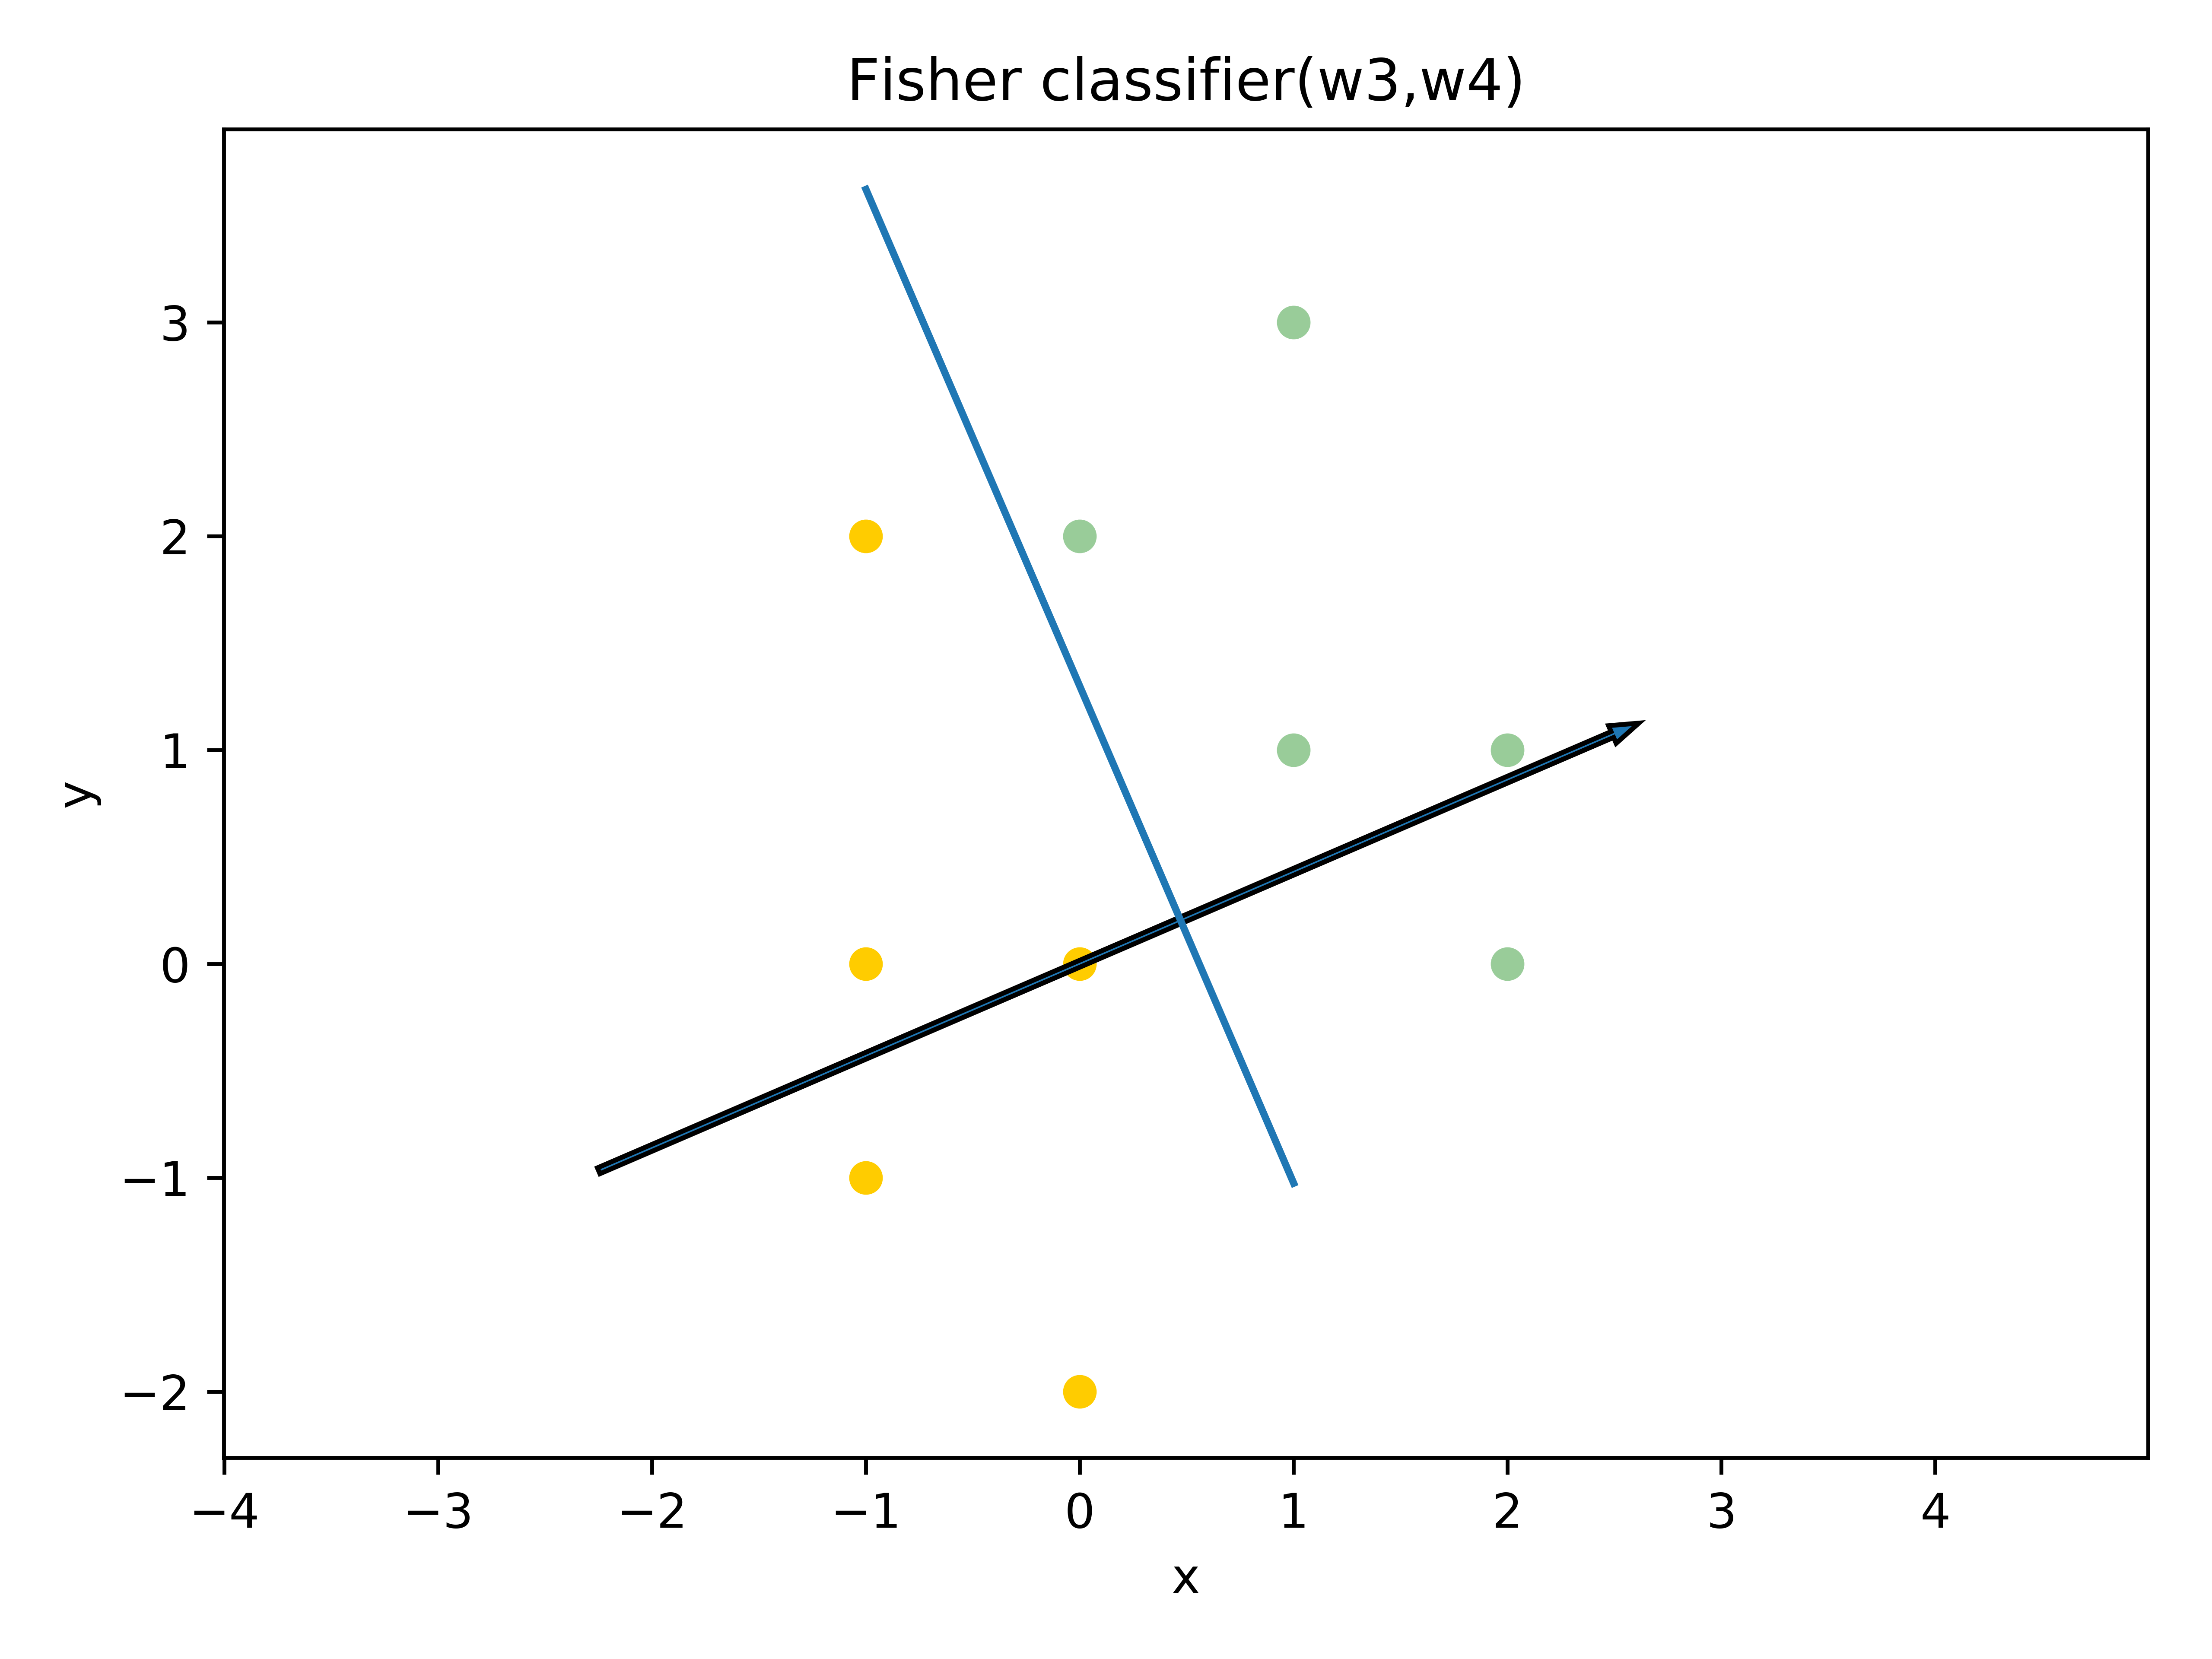
\includegraphics[width=0.6\linewidth]{img//fig11}
	\caption{Fisher判决的$w$和分界面}
\end{figure}

\subsection{Fisher实验结果分析}
\hs 对比图11和图12分析,我们发现Fisher判决,对于情况1来说,分类的效果并不是很好这一点可以观察数据就可以发现,显然在2维平面内这两类数据是线性不可分的;对于情况2,Fisher准则是一种很好的方法。它很好地区分了两类数据,究其原因也是因为情况2中的两类数据是线性可分的。
\end{document}
